% Compilazione: pdflatex -jobname=geometria_tex geometria.tex
\documentclass[11pt,a4paper]{article}
\usepackage[utf8]{inputenc}
\usepackage[T1]{fontenc}
\IfFileExists{italian.ldf}{\usepackage[italian]{babel}}{\usepackage[english]{babel}}
\usepackage{amsmath,amssymb,mathtools}
\usepackage[margin=2cm]{geometry}
\usepackage{hyperref}
\usepackage{graphicx}
\setlength{\parindent}{0pt}
\setlength{\emergencystretch}{3em}
\newcommand{\pagina}[1]{\clearpage}
\begin{document}
\begin{center}{\LARGE Geometria}\end{center}
% Pagina originale 1
\pagina{1}
\begin{flushleft}
LEGENDA\\
1. Relazioni\\
\textbullet{}     Definizione\\
\textbullet{}     Postulato\\
\textbullet{}     Teorema\\
\textbullet{}     Relazione d’equivalenza\\
\textbullet{}     Relazione d’ordine\\
\textbullet{}     Relazione funzionale\\
\par\smallskip
2. Funzioni\\
\textbullet{}     Iniettività\\
\textbullet{}     Suriettività\\
\textbullet{}     Biettività\\
\textbullet{}     Invertibilità\\
\textbullet{}     Composizione tra funzioni\\
\par\smallskip
3. Matrici\\
\textbullet{}     Matrici uguali\\
\textbullet{}     Matrice trasposta\\
\textbullet{}     Matrice simmetrica\\
\textbullet{}     Matrice antisimmetrica\\
\textbullet{}     Diagonale principale\\
\textbullet{}     Diagonale secondaria\\
\textbullet{}     Matrice nulla\\
\textbullet{}     Matrice identica\\
\textbullet{}     Sottomatrice\\
\textbullet{}     Minore complementare\\
\textbullet{}     Somma tra matrici\\
\textbullet{}     Prodotto per scalare\\
\textbullet{}     Prodotto righe per colonne\\
\textbullet{}     Matrice invertibile\\
\textbullet{}     Unicità matrice invertibile\\
\par\smallskip
4. Determinante\\
\textbullet{}     Cofattore\\
\textbullet{}     Matrice aggiunta\\
\textbullet{}     Primo th. di Laplace\\
\textbullet{}     Secondo th. di Laplace\\
\textbullet{}     |$A$ | = |$A$|\\
\textbullet{}     Th. di Binet\\
\textbullet{}     Matrici singolari\\
\textbullet{}     Combinazione lineare\\
\textbullet{}     Matrice triangolare\\
\textbullet{}     Matrice diagonale\\
\textbullet{}     Matrice scalare\\
\textbullet{}     Una matrice è invertibile se non singolare\\
\textbullet{}     Matrici permutabili\\
\textbullet{}     Matrice di permutazione\\
\textbullet{}     Matrici ortogonali\\
\par\smallskip
5. Rango\\
\textbullet{}     Minore fondamentale\\
\textbullet{}     Orlato\\
\textbullet{}     Th. degli orlati\\
\end{flushleft}
% Pagina originale 2
\pagina{2}
\begin{flushleft}
6. Eq. Lineari\\
\textbullet{}   Eq. lineari ad una incognita\\
\textbullet{}   Unicità soluzione lineare\\
\textbullet{}   Eq. lineari a due incognite\\
\textbullet{}   Eq. lineari omogenee\\
\textbullet{}   Eq. lineari ad n incognite\\
\textbullet{}   Eq. lineari equivalenti\\
\textbullet{}   Cosa rappresenta un’eq. lineare in R\textasciicircum{}n\\
\textbullet{}   Verifica equivalenza usando il rango\\
\par\smallskip
7. Sistemi Lineari\\
\textbullet{}   Matrice dei coe .\\
\textbullet{}   Matrice completa\\
\textbullet{}   Eq. linearmente dipendente dal sistema\\
\textbullet{}   Sistemi equivalenti\\
\textbullet{}   Th. di Rouché-Capelli\\
\textbullet{}   Sistema di Cramer\\
\textbullet{}   Un sistema di Cramer ha una singola soluzione\\
\textbullet{}   Regola di Cramer\\
\textbullet{}   Sistemi non di Cramer\\
\textbullet{}   Sistemi lineari omogenei\\
\textbullet{}   Cosa rappresenta un sistema lineare?\\
\par\smallskip
8. Strutture algebriche\\
\textbullet{}   Operazione binaria interna\\
\textbullet{}   Gruppo\\
\textbullet{}   Gruppo abeliano\\
\textbullet{}   Campo\\
\par\smallskip
\par\smallskip
9. Spazi vettoriali\\
\textbullet{}   Vettori linearmente dipendenti\\
\textbullet{}   Vettori linearmente indipendenti\\
\textbullet{}   Base di uno spazio vettoriale\\
\textbullet{}   Legame tra due basi\\
\textbullet{}   Ogni base ha lo stesso numero di elementi\\
\textbullet{}   Dimensione\\
\textbullet{}   Metodo degli scarti successivi\\
\textbullet{}   Completamento della base\\
\par\smallskip
\par\smallskip
10. Sottospazi vettoriali\\
\textbullet{}   Verifica del sottospazio\\
\textbullet{}   Sottospazio notevoli\\
\textbullet{}   Intersezione tra sottospazi\\
\textbullet{}   Unione tra sottospazi\\
\textbullet{}   Sottospazio somma\\
\textbullet{}   Spazi supplementari\\
\textbullet{}   Relazione di Grassmann\\
\par\smallskip
\par\smallskip
11. Applicazione lineare\\
\textbullet{}   Endomorfismo\\
\textbullet{}   Isomorfismo\\
\textbullet{}   Rappresentazione matriciale\\
\end{flushleft}
% Pagina originale 3
\pagina{3}
\begin{flushleft}
\textbullet{}   Proprietà delle appl. Lineari\\
\textbullet{}   Ker(f)\\
\textbullet{}   Im(f)\\
\textbullet{}   Un’appl. Lineare trasforma sottospazi in sottospazi\\
Applicazioni lineari: iniettività, nucleo e conservazione della lineare indipendenza.\\
Applicazioni lineari: iniettività, nucleo e conservazione della lineare indipendenza.\\
\textbullet{}   Teorema del rango\\
\textbullet{}   Generatori di Im(f)\\
\textbullet{}   Th. di esistenza e unicità\\
\par\smallskip
\par\smallskip
12. Vettori liberi\\
\textbullet{}   Relazione di equipollenza\\
\textbullet{}   Classe di equipollenza\\
\textbullet{}   Lunghezza del vettore\\
\textbullet{}   Vettore applicato\\
\textbullet{}   Prodotto per scalare\\
\textbullet{}   Vettori liberi nel piano\\
\textbullet{}   Vettori liberi nello spazio\\
\textbullet{}   Lineare dipendenza\\
\par\smallskip
\par\smallskip
13. Prodotto tra vettori\\
\textbullet{}   Prodotto scalare\\
\textbullet{}   Prodotto vettoriale\\
\textbullet{}   Prodotto misto\\
\par\smallskip
\par\smallskip
14. Autovalori\\
\textbullet{}   Intersezione tra due autospazi è sempre banale\\
\textbullet{}   Matrici simili\\
\textbullet{}   Matrice diagonalizzabile\\
\textbullet{}   Autovalori per una matrice\\
\textbullet{}   Polinomio caratteristico\\
\textbullet{}   Matrici simili hanno stesso polinomio caratteristico\\
\textbullet{}   Molteplicità algebrica\\
\textbullet{}   Molteplicità geometrica\\
\par\smallskip
\par\smallskip
15. Geometria\\
\textbullet{}   Riferimento cartesiano\\
\textbullet{}   Nella retta\\
\textbullet{}   Punto medio\\
\textbullet{}   Punto simmetrico\\
\textbullet{}   Nel piano\\
\textbullet{}   Nello spazio\\
\textbullet{}   Eq. parametrica della retta nello spazio\\
\textbullet{}   Allineamento di tre punti\\
\textbullet{}   Eq. della retta sotto forma di rapporti uguali\\
\textbullet{}   Parametri direttori\\
\textbullet{}   Rappresentazione della retta nel piano\\
\textbullet{}   Intersezioni e parallelismo tra due rette di un piano\\
\textbullet{}   Fascio proprio di rette\\
\end{flushleft}
% Pagina originale 4
\pagina{4}
\begin{flushleft}
\textbullet{}   Rette perpendicolari\\
\textbullet{}   Distanze nel piano\\
\textbullet{}   Coniche\\
\textbullet{}   Equazioni di un piano\\
\textbullet{}   Intersezioni e parallelismo tra piano\\
\textbullet{}   Fasci propri e impropri di piani\\
\textbullet{}   Intersezione tra piano e retta\\
\textbullet{}   Rette complanari e sghembe\\
\textbullet{}   Angoli tra rette nello spazio e tra piani\\
\textbullet{}   Distanza nello spazio\\
\textbullet{}   Minima distanza e retta di minima distanza\\
\end{flushleft}
% Pagina originale 5
\pagina{5}
\textbf{Definizione.} Nome assegnato ad un certo oggetto o ad una certa situazione.

\textbf{Postulato.} Nome dato ad un'affermazione che non ha bisogno di essere dimostrata poiché regola.

\textbf{Teorema.} Affermazione che necessita di dimostrazione poiché conseguenza dell'ipotesi.

\subsection*{Relazione d'equivalenza $(=)$}
$A\ne\varnothing$, $R\subseteq A\times A$:
\begin{enumerate}
\item $aRb\Longleftrightarrow bRa$: simmetrica;
\item $\forall a\in A: aRa$: riflessiva;
\item $aRb\wedge bRc\Longrightarrow aRc$: transitiva.
\end{enumerate}
\[ [a]:=\{x\in A\mid aRx\}. \]
Classe di equivalenza (esempio: $\frac12,\frac24,\ldots,\frac{k}{2k}$).
Insieme quoziente: $A/R:=\{[a]\text{ classe d'equivalenza}\}$.
\[ aRb\Longrightarrow[a]=[b],\qquad \bigcup_{[x]\in A/R}[x]=A,\qquad \varnothing\notin A/R.\]
\subsection*{Relazione d'ordine $(\le)$}
$A\ne\varnothing$, $R\subseteq A\times A$:
\begin{enumerate}
\item $\forall a\in A\Longrightarrow aRa$: riflessiva;
\item $aRb,\ bRa\Longrightarrow a=b$: antisimmetrica;
\item $aRb\wedge bRc\Longrightarrow aRc$: transitiva.
\end{enumerate}
% Pagina originale 6
\pagina{6}
\subsection*{Relazione funzionale}
$A\ne\varnothing\wedge B\ne\varnothing$, $R\subseteq A\times B$ tale che
\[\forall x\in A\quad\exists!y\in B:\ xRy.\]
\subsection*{Funzioni}
$f=(A,B,R)$: terna ordinata.
\[f:A\longrightarrow B,\quad R\subseteq A\times B,\qquad
\forall x\in A:\exists!y\in B\text{ tale che }xRy.\]
$f(x)=y$: $y$ è l'immagine; $x$ è una controimmagine.

\textbf{Iniettività:} $x_1\ne x_2\Longrightarrow f(x_1)\ne f(x_2)$;
$f(x_1)=f(x_2)\Longrightarrow x_1=x_2$.

\textbf{Suriettività:} $\forall y\in B\ \exists x\in A:\ y=f(x)$.

\textbf{Biettività:} $\forall y\in B\ \exists!x\in A:\ y=f(x)$.

\textbf{Invertibilità:} $f\circ f^{-1}=f^{-1}\circ f=x$, con $f=f(x)$ e $f^{-1}=f^{-1}(x)$ [notazione dell'originale].

\textbf{Composizione tra funzioni.} $A,B,C\ne\varnothing$:
\[ f:A\to B,\quad g:B\to C,\quad g\circ f:A\to C,\quad(g\circ f)(x)=g(f(x)).\]
% Pagina originale 7
\pagina{7}
\[g\circ f\ne f\circ g\quad\text{(non commutativa)},\qquad
 g\circ(f\circ h)=(g\circ f)\circ h\quad\text{(associativa)}.\]
\[f\circ f^{-1}=\operatorname{id}_A:A\to A,\quad
\forall x\in A:\operatorname{id}_A(x)=x.\]
\subsection*{Matrici}
Una matrice è una tabella $m\times n$ (con $m,n$ numeri naturali $>0$) di $mn$ numeri reali, disposti su $m$ righe ed $n$ colonne. In generale appartengono ad un campo qualsiasi.
\[A=\begin{pmatrix}a_{11}&a_{12}&a_{13}&\cdots&a_{1n}\\a_{21}&a_{22}&a_{23}&\cdots&a_{2n}\\\vdots&\vdots&\vdots&&\vdots\\a_{m1}&a_{m2}&a_{m3}&\cdots&a_{mn}\end{pmatrix}=(a_{ij}),\quad i\in\{1,\ldots,m\},\ j\in\{1,\ldots,n\}.\]
Se $m=n$, $A$ è matrice quadrata; se $m\ne n$, è matrice rettangolare.

\textbf{Matrici uguali.} Siano $A,B\in\mathbb R^{m,n}$:
\[ A=B\Longleftrightarrow\forall i=1,\ldots,m\ \forall j=1,\ldots,n:\ a_{ij}=b_{ij}.\]
\textbf{Matrice trasposta.} Sia $A\in\mathbb R^{m,n}$. Esiste $A^T\in\mathbb R^{n,m}$ tale che $a_{ij}=t_{ji}$, con $t\in A^T$.
\[(A^T)^T=A.\]
\textbf{Matrice simmetrica.} Sia $A=(a_{ij})\in\mathbb R^{m,m}$. Se $\forall i,j\in\{1,\ldots,m\}:a_{ij}=a_{ji}$, $A$ è detta simmetrica.
Se $A$ è simmetrica, $A=A^T\wedge A^T=A$. Se $A\in\mathbb R^{m,n}$ e $m\ne n$, $A$ non può essere simmetrica.
% Pagina originale 8
\pagina{8}
\textbf{Matrice antisimmetrica.} Sia $A\in\mathbb R^{m,m}$. Se $\forall i,j\in\{1,\ldots,m\}:a_{ij}=-a_{ji}$, $A$ è antisimmetrica. Se esiste un elemento della diagonale principale $d_k\ne0$, $A$ non può essere antisimmetrica.

\textbf{Diagonale principale.} È la $m$-upla di elementi con indici uguali: $(a_{11},a_{22},\ldots,a_{mm})$.

\textbf{Diagonale secondaria.} È la $m$-upla di elementi la cui somma degli indici fa $m+1$: $(a_{1m},a_{2,m-1},\ldots,a_{m1})$.

\textbf{Matrice nulla.} Matrice con tutti gli elementi uguali a $0$:
\[O_{m,n}\in\mathbb R^{m,n},\qquad\forall i\in\{1,\ldots,m\},j\in\{1,\ldots,n\}:a_{ij}=0.\]
\textbf{Matrice identica.} $\operatorname{Id}_m$, una matrice dove
\[i_{ij}=\begin{cases}1&\text{se }i=j,\\0&\text{se }i\ne j.\end{cases}\]
\textbf{Sottomatrice.} Sia $A=(a_{ij})\in\mathbb R^{m,n}$. Togliendo ad $A$ $h$ righe e $k$ colonne si ottiene una matrice $A'=(a'_{ij})\in\mathbb R^{m-h,n-k}$, chiamata matrice estratta o sottomatrice. Se $m-h=n-k$, la sottomatrice viene detta minore estratto.

\textbf{Minore complementare.} Sia $A=(a_{ij})\in\mathbb R^{n,n}$. $M_{ij}$ è il minore estratto da $A$ togliendo la riga $i$ e la colonna $j$; $M_{ij}\in\mathbb R^{n-1,n-1}$.
% Pagina originale 9
\pagina{9}
\subsection*{Operazioni tra matrici}
$A+B$ si chiama somma tra matrici:
\[A=(a_{ij}),\quad B=(b_{ij}),\quad A+B=(a_{ij}+b_{ij}).\]
\textbf{Addizione.} La somma verifica alcune proprietà:
\begin{enumerate}
\item $\forall A,B,C\in\mathbb R^{m,n}: (A+B)+C=A+(B+C)$;
\item $\exists O_{m,n}\in\mathbb R^{m,n}:\forall A\in\mathbb R^{m,n},\ A+O_{m,n}=A$;
\item $\forall A\in\mathbb R^{m,n}:\exists B\in\mathbb R^{m,n}:A+B=O_{m,n}$;
\item $\forall A,B\in\mathbb R^{m,n}:A+B=B+A$.
\end{enumerate}
Soddisfa quindi la proprietà associativa, l'esistenza dell'elemento neutro, l'opposto e la proprietà commutativa.
La matrice opposta è unica per ogni matrice. Supponiamo per assurdo $C\ne B$, con $B$ e $C$ matrici opposte di $A$:
\[C=C+O_{m,n}=C+(A+B)=(C+A)+B=O_{m,n}+B=B.\]
Da cui deriva $C=B$: abbiamo dimostrato l'unicità della matrice opposta, denotata come $-A$.

\textbf{Prodotto con scalare.} Sia $A=(a_{ij})\in\mathbb R^{m,n}$ e $h\in\mathbb R$ scalare: $hA=(ha_{ij})$.
% Pagina originale 10
\pagina{10}
Soddisfa alcune proprietà:
\begin{enumerate}
\item $\forall h\in\mathbb R,\ \forall A,B\in\mathbb R^{m,n}:h(A+B)=hA+hB$;
\item $\forall h,k\in\mathbb R,\ \forall A\in\mathbb R^{m,n}:(h+k)A=hA+kA$;
\item $\forall h,k\in\mathbb R,\ \forall A\in\mathbb R^{m,n}:(hk)A=h(kA)$;
\item $\forall A\in\mathbb R^{m,n}:1A=A$.
\end{enumerate}
Che sono: distributiva rispetto alla somma di matrici, distributiva rispetto alla somma di scalari, associativa ed esistenza dell'elemento ``neutro''. $Ah$ non ha significato, quindi non c'è proprietà commutativa. Non esiste un vero e proprio elemento neutro, quindi non esiste un simmetrico.

\textbf{Prodotto righe per colonne.} Siano $A=(a_{ij})\in\mathbb R^{m,n}$, $B=(b_{jk})\in\mathbb R^{n,q}$:
\[AB=(c_{ik})\in\mathbb R^{m,q},\qquad c_{ik}=\sum_{j=1}^n a_{ij}b_{jk}=a_{i1}b_{1k}+a_{i2}b_{2k}+\cdots+a_{in}b_{nk}.\]
Proprietà:
\begin{enumerate}
\item $(AB)C=A(BC)$: associativa;
\item $A(B+C)=AB+AC$;
\item $(A+B)C=AC+BC$: distributiva;
\item $h(AB)=(hA)B=A(hB)$;
\item $(AB)^T=B^TA^T$;
\item $\forall A\in\mathbb R^{m,n}:AI_n=I_mA=A$.
\end{enumerate}
% Pagina originale 11
\pagina{11}
\textbf{Matrice invertibile.} $A=(a_{ij})\in\mathbb R^{n,n}$ è invertibile se esiste $B\in\mathbb R^{n,n}$ tale che $AB=I_n\wedge BA=I_n$. $B$ è detta (se esiste) $A^{-1}$.

\textbf{Unicità matrice inversa.} Per assurdo supponiamo ci siano due matrici inverse di $A$ (matrice invertibile di ordine $n$), $B$ e $C$:
\[B=BI_n=B(AC)=(BA)C=I_nC=C.\]
$B=C$, quindi devono necessariamente coincidere.
\subsection*{Determinante}
È un numero reale associato alla matrice. Può essere calcolato esclusivamente nelle matrici quadrate.
\[A=(a_{11})\Longrightarrow\det A=a_{11}.\]
\[A=\begin{pmatrix}a_{11}&a_{12}\\a_{21}&a_{22}\end{pmatrix}\Longrightarrow\det A=a_{11}a_{22}-a_{12}a_{21}.\]
Per $A\in\mathbb R^{m,m}$ con $m\ge3$ si usa il metodo di Laplace (per $m=3$ anche quello di Sarrus è molto utilizzato).
La formula generale per il calcolo del determinante è:
\[\det A=\sum_{i=1}^m(-1)^{i+j}a_{ij}\det(M_{ij}).\]
% Pagina originale 12
\pagina{12}
$(-1)^{i+j}\det(M_{ij})=A_{ij}$, detto complemento algebrico dell'elemento $a_{ij}$; quindi
\[\det A=\sum_{i=1}^m(-1)^{i+j}a_{ij}\det(M_{ij})=\sum_{i=1}^m a_{ij}A_{ij}.\]
Si può anche fissare $i$, quindi $\det A=\sum_{j=1}^m a_{ij}A_{ij}$.

\textbf{Cofattore} di $a_{ij}$: $A_{ij}=(-1)^{i+j}\det M_{ij}$.

\textbf{Matrice aggiunta.} $\operatorname{Agg}(A)\in\mathbb R^{m,m}$,
$\operatorname{Agg}(A)=(A_{ji})$: $ji$ e non $ij$.

\textbf{Primo teorema di Laplace.} $|A|$ è uguale alla somma dei prodotti degli elementi di una qualsiasi riga/colonna per i propri complementi algebrici:
\[|A|=a_{1j}A_{1j}+a_{2j}A_{2j}+\cdots+a_{mj}A_{mj},\quad\forall j\in\{1,\ldots,m\},\]
\[|A|=a_{i1}A_{i1}+a_{i2}A_{i2}+\cdots+a_{im}A_{im},\quad\forall i\in\{1,\ldots,m\}.\]
\textbf{Secondo teorema di Laplace.} La somma dei prodotti degli elementi di una qualsiasi riga/colonna per i complementi algebrici di un'altra riga/colonna è sempre nulla.
% Pagina originale 13
\pagina{13}
\[\sum_{i=1}^m a_{ij}A_{ik}=0\quad\forall j,k\in\{1,\ldots,m\},\ j\ne k,\qquad
\sum_{j=1}^m a_{ij}A_{hj}=0\quad\forall i,h\in\{1,\ldots,m\},\ i\ne h.\]
\textbf{$|A^T|=|A|$.} Si dimostra notando che il calcolo del determinante di $A^T$ sviluppato nella prima riga coincide con quello sviluppato nella prima colonna in $A$.
Scambiando due righe o due colonne si ha $|A'|=-|A|$. Se scambiamo due righe uguali, $A'=A$ e $|A'|=-|A|$, quindi $|A|=0$.

\textbf{Teorema di Binet:} $|AB|=|A||B|$.
Proprietà del determinante:
\[\begin{vmatrix}b_{11}+c_{11}&b_{12}+c_{12}&\cdots&b_{1m}+c_{1m}\\a_{21}&a_{22}&\cdots&a_{2m}\\\vdots&\vdots&&\vdots\\a_{m1}&a_{m2}&\cdots&a_{mm}\end{vmatrix}
=\begin{vmatrix}b_{11}&b_{12}&\cdots&b_{1m}\\a_{21}&a_{22}&\cdots&a_{2m}\\\vdots&\vdots&&\vdots\\a_{m1}&a_{m2}&\cdots&a_{mm}\end{vmatrix}
+\begin{vmatrix}c_{11}&c_{12}&\cdots&c_{1m}\\a_{21}&a_{22}&\cdots&a_{2m}\\\vdots&\vdots&&\vdots\\a_{m1}&a_{m2}&\cdots&a_{mm}\end{vmatrix}.\]
\[\begin{vmatrix}ha_{11}&ha_{12}&\cdots&ha_{1m}\\a_{21}&a_{22}&\cdots&a_{2m}\\\vdots&\vdots&&\vdots\\a_{m1}&a_{m2}&\cdots&a_{mm}\end{vmatrix}
=h\begin{vmatrix}a_{11}&a_{12}&\cdots&a_{1m}\\a_{21}&a_{22}&\cdots&a_{2m}\\\vdots&\vdots&&\vdots\\a_{m1}&a_{m2}&\cdots&a_{mm}\end{vmatrix}.\]
Sono dette proprietà di multilinearità. Se c'è una riga/colonna composta solo da $0$, allora $|A|=0$.
\[\begin{vmatrix}ha&hb&\cdots&hm\\a&b&\cdots&m\\\vdots&\vdots&&\vdots\end{vmatrix}
=h\begin{vmatrix}a&b&\cdots&m\\a&b&\cdots&m\\\vdots&\vdots&&\vdots\end{vmatrix}=0.\]
Questo se sono righe/colonne proporzionali.
% Pagina originale 14
\pagina{14}
\textbf{Matrici singolari.} $A=(a_{ij})\in\mathbb R^{m,m}$ è singolare o degenere se $|A|=0$. Se $|A|\ne0$, $A$ è non singolare.

\textbf{Combinazione lineare.} Una riga/colonna è combinazione lineare di altre righe/colonne se si ottiene dalla somma di quelle righe moltiplicate per dei coefficienti. Se una riga/colonna è combinazione lineare allora è linearmente dipendente.
Esistono $h_1,h_2,\ldots,h_{m-1}\in\mathbb R$ tali che
\begin{align*}
a_{m1}&=h_1a_{11}+h_2a_{21}+h_3a_{31}+\cdots+h_{m-1}a_{m-1,1},\\
a_{m2}&=h_1a_{12}+h_2a_{22}+h_3a_{32}+\cdots+h_{m-1}a_{m-1,2},\\&\vdots\\
a_{mm}&=h_1a_{1m}+h_2a_{2m}+h_3a_{3m}+\cdots+h_{m-1}a_{m-1,m}.
\end{align*}
La riga $m$ è combinazione lineare. Possiamo riassumere molte proprietà in un semplice teorema:
una matrice $A\in\mathbb R^{m,m}$ è singolare se esiste una riga/colonna combinazione lineare di altre righe/colonne.

\textbf{Matrice triangolare.} Bassa: $a_{ij}=0$ se $i<j$; alta: $a_{ij}=0$ se $i>j$.
\[\begin{pmatrix}1&0&0\\4&2&0\\5&6&3\end{pmatrix}\quad\text{bassa},\qquad
\begin{pmatrix}1&4&0\\0&2&7\\0&0&3\end{pmatrix}\quad\text{alta}.\]
% Pagina originale 15
\pagina{15}
\textbf{Matrice diagonale.} $a_{ij}=0$ se $i\ne j$: triangolare bassa e triangolare alta.
\[\begin{pmatrix}0&0&0\\0&3&0\\0&0&5\end{pmatrix}.\]
\textbf{Matrice scalare.} $\forall i,j\in\{1,\ldots,m\}:a_{ij}=k$, $i=j$. Tutti gli elementi della diagonale principale sono uguali tra loro.
Nell'originale è disegnata $\begin{pmatrix}k&1&1\\2&k&2\\3&0&k\end{pmatrix}$ [esempio riportato fedelmente, pur non diagonale].

\textbf{Una matrice è invertibile se $\det A\ne0$.}
Se $AA^{-1}=I_m$, allora $\det(AA^{-1})=\det(A)\det(A^{-1})$;
\[\det I_m=1=\det(A)\det(A^{-1}),\qquad \det(A^{-1})=\frac1{\det A}.\]
\[I_m=\frac1{|A|}(A\operatorname{Agg}A),\quad\text{poiché}\quad
A\operatorname{Agg}A=\begin{pmatrix}|A|&0&\cdots&0\\0&|A|&\cdots&0\\\vdots&\vdots&\ddots&\vdots\\0&0&\cdots&|A|\end{pmatrix}.\]
Quindi $I_m=(\frac1{|A|}\operatorname{Agg}A)A$ e $I_m=BA\Longleftrightarrow B=\frac1{|A|}\operatorname{Agg}A=A^{-1}$.
$A$ invertibile, $B$ invertibile $\Longrightarrow AB$ invertibile. Dal teorema di Binet $|A||B|=|AB|$, e $|A|\ne0\wedge|B|\ne0$, quindi $|AB|\ne0$.
% Pagina originale 16
\pagina{16}
$GL(m,\mathbb R)$ è il gruppo lineare generale:
\[GL(m,\mathbb R):=\{A\in\mathbb R^{m,m}\mid A\text{ è invertibile}\}.\]
Proprietà:
\begin{enumerate}
\item $\forall A,B,C\in GL(m,\mathbb R):A(BC)=(AB)C$ (associativa);
\item $\forall A\in GL(m,\mathbb R):I_mA=AI_m=A$ (elemento neutro);
\item $\forall A\in GL(m,\mathbb R)\ \exists A^{-1}\in GL(m,\mathbb R):AA^{-1}=A^{-1}A=I_m$ (simmetrico).
\end{enumerate}
Non vale la proprietà commutativa.

\textbf{Matrici permutabili.} $A,B\in\mathbb R^{m,m}$ sono permutabili se $AB=BA$. $O_{m,m}$ e $I_m$ sono permutabili con qualsiasi matrice. $A$ e $A^{-1}$ sono permutabili tra loro.

\textbf{Matrice di permutazione.} $A\in\mathbb R^{m,m}$ che ha un solo elemento $=1$ per ogni riga/colonna.
\[P=\begin{pmatrix}0&1&0\\1&0&0\\0&0&1\end{pmatrix},\quad|P|=-1,\qquad
PA=\begin{pmatrix}a_{21}&a_{22}&a_{23}\\a_{11}&a_{12}&a_{13}\\a_{31}&a_{32}&a_{33}\end{pmatrix}.\]
La figura indica lo scambio delle prime due righe e la terza invariata.

\textbf{Matrici ortogonali.} $A\in\mathbb R^{m,m}$ ortogonale se $AA^T=A^TA=I_m$.
% Pagina originale 17
\pagina{17}
$A$ ortogonale $\Longrightarrow A^T=A^{-1}$, quindi $A$ invertibile.
$A$ ortogonale $\Longrightarrow\det A=1\vee\det A=-1$:
\[AA^T=I_m\Longrightarrow|A||A^T|=|I_m|\Longrightarrow|A|^2=1\Longrightarrow|A|=1\vee|A|=-1.\]
$A$ ortogonale se e solo se
\[\sum_{j=1}^m(a_{ij})^2=1\quad\forall i\in\{1,\ldots,m\},\qquad
\sum_{j=1}^m a_{ij}a_{kj}=0\quad\forall i,k\in\{1,\ldots,m\},\ i\ne k.\]
Vale anche per le colonne. Esempi di matrici ortogonali sono quelle di permutazione e $\begin{pmatrix}\sin\varphi&-\cos\varphi\\\cos\varphi&\sin\varphi\end{pmatrix}$.
$O(m,\mathbb R)$ è il sottogruppo ortogonale:
\[O(m,\mathbb R):=\{A\in GL(m,\mathbb R)\mid A\text{ ortogonale}\}.\]
\subsection*{Rango}
È l'ordine massimo di minori non singolari estratti da $A$.
$A=O_{m,n}\Longrightarrow r(A)=0$ per convenzione.

\textbf{Minore fondamentale.} Uno dei minori che determina il rango di $A$: $|M|\ne0$, $M\in\mathbb R^{p,p}$ con $p=r(A)$.
% Pagina originale 18
\pagina{18}
\textbf{Orlato.} Sia $M$ minore di $A\in\mathbb R^{m,n}$. $O_M$ è un orlato di $M$ se ad $M$, matrice di ordine $p$, aggiungiamo una qualsiasi altra riga e una qualsiasi altra colonna di $A$.

\textbf{Teorema degli orlati.} $r(A)=p$ se e solo se
\begin{enumerate}
\item esiste $M$ minore estratto di $A$ di ordine $p$ con $|M|\ne0$;
\item per ogni $O$ orlato di $M$, $|O|=0$.
\end{enumerate}
\textbf{Matrici con parametro.} Una matrice contenente uno o più parametri indica un'infinità di matrici, a seconda dei valori dati ai parametri.
\subsection*{Equazioni lineari ad una incognita}
\[S=\{x\in\mathbb R\mid ax=b\},\qquad a,b\in\mathbb R.\]
Se $a=0$: $b=0\Longrightarrow S=\mathbb R$; $b\ne0\Longrightarrow S=\varnothing$.
Se $a\ne0$, esiste $a^{-1}=1/a$ e $x=a^{-1}b$, quindi $S=\{a^{-1}b\}$.

\textbf{Unicità soluzione lineare.} Siano $x_1,x_2\in S$:
\[ax_1=ax_2\Longrightarrow a(x_1-x_2)=0\Longrightarrow x_1=x_2.\]
% Pagina originale 19
\pagina{19}
\subsection*{Equazioni lineari a due incognite}
\[S=\{(x_1,x_2)\in\mathbb R^2\mid a_1x_1+a_2x_2=b\}.\]
Se $(a_1,a_2)=(0,0)$: $b=0\Longrightarrow S=\mathbb R^2$; $b\ne0\Longrightarrow S=\varnothing$.
Se $a_1\ne0$: $x_2=h_2$, $a_1x_1+a_2h_2=b\Longrightarrow x_1=a_1^{-1}(b-a_2h_2)$:
\[S_1=\{(a_1^{-1}(b-a_2h_2),h_2)\in\mathbb R^2\mid h_2\in\mathbb R\}.\]
Se $a_2\ne0$: $x_1=k_1$, $a_1k_1+a_2x_2=b\Longrightarrow x_2=a_2^{-1}(b-a_1k_1)$:
\[S_2=\{(k_1,a_2^{-1}(b-a_1k_1))\in\mathbb R^2\mid k_1\in\mathbb R\}.\]
$S_1=S_2\Longleftrightarrow S_1\subseteq S_2\wedge S_2\subseteq S_1$.
Prendo $(a_1^{-1}(b-a_2h_2),h_2)\in S_1$. Pongo $k_1=a_1^{-1}(b-a_2h_2)$:
\begin{align*}
x_2&=a_2^{-1}(b-a_1k_1)=a_2^{-1}(b-a_1a_1^{-1}(b-a_2h_2))\\
&=a_2^{-1}(b-b+a_2h_2)=a_2^{-1}a_2h_2=h_2.
\end{align*}
\textbf{Equazione lineare omogenea.} Se $b=0$ in $S$:
\begin{enumerate}
\item $(0,0)\in S$: soluzione banale;
\item $(y_1,y_2)\in S\wedge(z_1,z_2)\in S\Longrightarrow(y_1+z_1,y_2+z_2)\in S$;
\item $(y_1,y_2)\in S\Longrightarrow h(y_1,y_2)=(hy_1,hy_2)\in S$.
\end{enumerate}
% Pagina originale 20
\pagina{20}
Dimostrazione del punto 2: $a_1y_1+a_2y_2=0\wedge a_1z_1+a_2z_2=0$:
\begin{align*}
a_1(y_1+z_1)+a_2(y_2+z_2)&=a_1y_1+a_2y_2+a_1z_1+a_2z_2\\
&=(a_1y_1+a_2y_2)+(a_1z_1+a_2z_2)=0+0=0.
\end{align*}
Punto 3: $a_1y_1+a_2y_2=0$, $h\in\mathbb R$:
\[a_1(hy_1)+a_2(hy_2)=ha_1y_1+ha_2y_2=h(a_1y_1+a_2y_2)=h\cdot0=0.\]
\subsection*{Equazioni lineari in $n$ incognite}
\[S=\{(x_1,x_2,\ldots,x_n)\in\mathbb R^n\mid a_1x_1+a_2x_2+\cdots+a_nx_n=b\}.\]
Se $(a_1,\ldots,a_n)=(0,\ldots,0)$: $b=0\Longrightarrow S=\mathbb R^n$; $b\ne0\Longrightarrow S=\varnothing$.
Se $(a_1,\ldots,a_n)\ne(0,\ldots,0)$, sia $a_m\ne0$:
\[x_m=a_m^{-1}\left(b-\sum_{i\in N}a_ik_i\right),\qquad N=\{1,\ldots,n\}\setminus\{m\}.\]
Verifichiamo la soluzione:
\[a_ma_m^{-1}\left(b-\sum_{i\ne m}a_ik_i\right)+\sum_{i\ne m}a_ik_i=b.\]
Quindi $S=\{(k_1,\ldots,k_{m-1},a_m^{-1}(b-\sum_{i\ne m}a_ik_i),k_{m+1},\ldots,k_n)\}$.
Le soluzioni sono $\infty^{n-1}$: infinite soluzioni che dipendono da $n-1$ parametri.
% Pagina originale 21
\pagina{21}
\textbf{Equazioni lineari equivalenti.}
\[S_1=\{x\in\mathbb R^n\mid a_1x_1+\cdots+a_nx_n=c\},\quad S_2=\{x\in\mathbb R^n\mid b_1x_1+\cdots+b_nx_n=d\}.\]
$S_1=S_2$ se e solo se sono proporzionali: esiste $h\in\mathbb R^*$ tale che $b_1=ha_1,\ldots,b_n=ha_n,d=hc$.
($\Leftarrow$) Se $u\in S_1$, $\sum a_iu_i=c\Longrightarrow h\sum a_iu_i=hc\Longrightarrow\sum b_iu_i=d$, quindi $u\in S_2$. Se $v\in S_2$, $\sum b_iv_i=d\Longrightarrow h^{-1}\sum b_iv_i=h^{-1}d\Longrightarrow\sum a_iv_i=c$, quindi $v\in S_1$.
($\Rightarrow$) $h=d/c\Longrightarrow d=hc$ nel caso di equazioni non omogenee. $a_1\ne0\Longrightarrow b_1\ne0$. Pongo $x_2=\cdots=x_n=0$, quindi $a_1x_1=c$ e $(a_1^{-1}c,0,\ldots,0)\in S_1\cap S_2$. Quindi $b_1(a_1^{-1}c)=d=hc\Longrightarrow h=a_1^{-1}b_1\Longrightarrow b_1=ha_1$. Questo ragionamento è applicabile prendendo
% Pagina originale 22
\pagina{22}
qualsiasi indice $j\in\{1,\ldots,n\}$ tale che $a_j\ne0\wedge b_j\ne0$.
Nel caso delle equazioni omogenee: se $a_1\ne0$, allora $b_1\ne0$. Se $b_1=0$, $(1,0,\ldots,0)\in S_2$ e quindi $a_1\cdot1+a_2\cdot0+\cdots+a_n\cdot0=0\Longrightarrow a_1=0$. Possiamo applicare lo stesso ragionamento per qualsiasi indice $j$ tale che $a_j\ne0\wedge b_j\ne0$.
Possiamo trasformare un'equazione lineare omogenea ad $n$ incognite in una ad $n-1$ incognite con termine noto $a_j,b_j$, tali che $a_j\ne0\wedge b_j\ne0$:
\[S_1=\{x\in\mathbb R^n\mid a_1x_1+\cdots+a_nx_n=0\}\]
diventa
\[S'_1=\{(x_1,\ldots,x_{n-1})\in\mathbb R^{n-1}\mid a_1x_1+\cdots+a_{n-1}x_{n-1}=-a_n\},\]
assegnando ad $x_n$ il valore $1$. P.S. Questo caso non va bene se $a_n,b_n$ sono gli unici coefficienti non nulli. In questo caso abbiamo $a_nx_n=0\wedge b_nx_n=0$, con $a_n\ne0\wedge b_n\ne0$, quindi $h=a_nb_n^{-1}$ [rapporto riportato nell'originale].

\textbf{Cosa rappresenta un'equazione lineare in $\mathbb R^n$?} Rappresenta un iperpiano nello spazio geometrico
% Pagina originale 23
\pagina{23}
di dimensione $n$. Nel piano un iperpiano è una retta ($\infty^1$), nello spazio un piano ($\infty^2$), in quattro dimensioni uno spazio geometrico ($\infty^3$), ecc.

\textbf{Verifica equivalenza usando il rango.}
\[M=\begin{pmatrix}a_1&a_2&\cdots&a_n&b\\c_1&c_2&\cdots&c_n&d\end{pmatrix}.\]
Matrice $2\times(n+1)$ contenente per prima riga i coefficienti della prima equazione e per seconda riga quelli della seconda. Se $r(M)=1$ (oppure $r(M)=0$, con $S_1=\mathbb R^n,S_2=\mathbb R^n\Longrightarrow S_1=S_2$), la prima riga è proporzionale alla seconda.
\subsection*{Sistemi lineari}
È formato da $m\ge1$, $m\in\mathbb N$, equazioni lineari:
\[\begin{cases}a_{11}x_1+a_{12}x_2+\cdots+a_{1n}x_n=b_1,\\a_{21}x_1+a_{22}x_2+\cdots+a_{2n}x_n=b_2,\\\vdots\\a_{m1}x_1+a_{m2}x_2+\cdots+a_{mn}x_n=b_m.\end{cases}\]
L'insieme delle soluzioni è l'intersezione tra gli insiemi di soluzione di tutte le $m$ equazioni lineari.
\textbf{Matrice dei coefficienti (incompleta).}
\[A=\begin{pmatrix}a_{11}&a_{12}&\cdots&a_{1n}\\a_{21}&a_{22}&\cdots&a_{2n}\\\vdots&\vdots&&\vdots\\a_{m1}&a_{m2}&\cdots&a_{mn}\end{pmatrix}\quad\text{di tipo }m\times n.\]
% Pagina originale 24
\pagina{24}
\textbf{Matrice completa.}
\[\bar A=\begin{pmatrix}a_{11}&a_{12}&\cdots&a_{1n}&b_1\\a_{21}&a_{22}&\cdots&a_{2n}&b_2\\\vdots&\vdots&&\vdots&\vdots\\a_{m1}&a_{m2}&\cdots&a_{mn}&b_m\end{pmatrix}\quad\text{di tipo }m\times(n+1).\]
Ad ogni sistema si possono associare le matrici incompleta e completa. Sia $A$ matrice incompleta, $X=(x_1,\ldots,x_n)^T$, $B=(b_1,\ldots,b_m)^T$: il sistema può essere scritto in forma matriciale $AX=B$.

\textbf{Equazione linearmente dipendente dal sistema.} $c_1x_1+\cdots+c_nx_n=d$ è linearmente dipendente dal sistema se esistono $(h_i)_{i\in\{1,\ldots,m\}}$ tali che
\[\forall j\in\{1,\ldots,n\}:c_j=h_1a_{1j}+\cdots+h_ma_{mj},\qquad d=h_1b_1+\cdots+h_mb_m.\]
\textbf{Sistemi equivalenti.} Due sistemi sono equivalenti se i rispettivi insiemi di soluzione coincidono.
\textbf{Teorema.} Due sistemi sono equivalenti se e solo se ciascuna equazione del primo sistema dipende linearmente dalle equazioni del secondo e viceversa.
% Pagina originale 25
\pagina{25}
\subsection*{Teorema di Rouché--Capelli}
1) Condizione necessaria e sufficiente affinché un sistema sia compatibile è che $r(A)=r(\bar A)$.
2) Un sistema compatibile ammette un'unica soluzione se $n$ (numero di incognite) $=p$, dove $p=r(A)=r(\bar A)$. Se $p<n$ il sistema ammette $\infty^{n-p}$ soluzioni.
\textbf{Sistema di Cramer.} Un sistema lineare di $n$ equazioni lineari in $n$ incognite con $|A|\ne0$.
\textbf{Un sistema è di Cramer $\Longleftrightarrow$ 1 soluzione.}
Dimostrazione: $|A|\ne0\Rightarrow r(A)=n$. Inoltre $r(\bar A)\ge r(A)$ e $r(\bar A)\le n$, quindi $r(\bar A)=n=r(A)$; $p=r(A)$ implica $n=p$, quindi ammette un'unica soluzione.
\textbf{Regola di Cramer.}
\[x_1=\frac{\begin{vmatrix}b_1&a_{12}&\cdots&a_{1n}\\b_2&a_{22}&\cdots&a_{2n}\\\vdots&\vdots&&\vdots\\b_n&a_{n2}&\cdots&a_{nn}\end{vmatrix}}{|A|},\quad x_2=\frac{\begin{vmatrix}a_{11}&b_1&\cdots&a_{1n}\\a_{21}&b_2&\cdots&a_{2n}\\\vdots&\vdots&&\vdots\\a_{n1}&b_n&\cdots&a_{nn}\end{vmatrix}}{|A|},\ldots\]
\textbf{Sistemi non di Cramer.} Per risolvere un sistema lineare non di Cramer bisogna prima effettuare il teorema di Rouché--Capelli. Sia $p=r(A)=r(\bar A)$ e $p<n$ (con $p=n$ il sistema è di Cramer): bisogna trovare uno
% Pagina originale 26
\pagina{26}
dei minori estratti $M$ con $|M|\ne0$ e che abbia per ordine il rango delle due matrici.
Bisogna riscrivere il nuovo sistema con solo le righe prese in considerazione da $M$ (questo sistema sarà equivalente a quello dato inizialmente). Bisogna trasformare $n-p$ incognite in parametri e le incognite che dovremo trasformare sono quelle delle colonne escluse.
\[\begin{cases}x+y+z=20,\\2x+y+\frac7{10}z=20,\end{cases}\quad A=\begin{pmatrix}1&1&1\\2&1&7/10\end{pmatrix},\quad\bar A=\begin{pmatrix}1&1&1&20\\2&1&7/10&20\end{pmatrix}.\]
\[r(A)=r(\bar A)=2,\quad M=\begin{pmatrix}1&1\\2&1\end{pmatrix},\quad |M|=-1\ne0.\]
Il nuovo sistema ha prima e seconda riga (che sono le uniche, quindi i due sistemi sono identici). La colonna 3 non è utilizzata: $z=h$.
\[\begin{cases}x+y=20-h,\\2x+y=20-\frac7{10}h\end{cases}\Rightarrow\begin{cases}x=\frac3{10}h,\\y=20-h-\frac3{10}h\end{cases}\Rightarrow\begin{cases}x=\frac3{10}h,\\y=20-\frac{13}{10}h.\end{cases}\]
\[S=\{(\tfrac3{10}h,20-\tfrac{13}{10}h,h)\in\mathbb R^3\mid h\in\mathbb R\}.\]
% Pagina originale 27
\pagina{27}
\subsection*{Sistemi lineari omogenei}
È un sistema lineare composto esclusivamente da equazioni lineari omogenee. Come anche le equazioni lineari omogenee: ammette sempre $(0,0,\ldots,0)$; se $\bar v_1,\bar v_2$ sono soluzioni, $\bar v_1+\bar v_2$ è soluzione; se $\bar v_1$ è soluzione, $h\bar v_1$ è soluzione.
Se un sistema di Cramer è omogeneo avrà come unica soluzione quella banale. $r(A)<n\Longleftrightarrow$ il sistema ammette altre soluzioni oltre a quella banale.
\textbf{Teorema.} Preso un sistema con $m$ equazioni lineari ed $m+1$ incognite con $r(A)=m$, una sua soluzione è (attenzione ai segni alterni)
\[\left(\begin{vmatrix}a_{12}&a_{13}&\cdots&a_{1,m+1}\\\vdots&\vdots&&\vdots\\a_{m2}&a_{m3}&\cdots&a_{m,m+1}\end{vmatrix},-\begin{vmatrix}a_{11}&a_{13}&\cdots&a_{1,m+1}\\\vdots&\vdots&&\vdots\\a_{m1}&a_{m3}&\cdots&a_{m,m+1}\end{vmatrix},\ldots,(-1)^m\begin{vmatrix}a_{11}&a_{12}&\cdots&a_{1m}\\\vdots&\vdots&&\vdots\\a_{m1}&a_{m2}&\cdots&a_{mm}\end{vmatrix}\right)\]
\[=(c_1,-c_2,c_3,\ldots,\pm c_{m+1}),\quad S=\{(hc_1,-hc_2,\ldots,\pm hc_{m+1})\in\mathbb R^{m+1}\mid h\in\mathbb R\}.\]
Il segno dipende da $m\bmod2$.
\textbf{Cosa rappresenta un sistema lineare?} Rappresenta l'intersezione tra gli iperpiani.
% Pagina originale 28
\pagina{28}
\section*{Strutture algebriche}
\textbf{Operazione binaria (interna).} Sia $G$ insieme non vuoto: si chiama $\omega$ una funzione $\omega:G\times G\to G$. La coppia $(G,\omega)$ si chiama struttura algebrica ed il valore che assume $\omega(a,b)$ si denota con $a\mathbin\omega b$ (composto di $a,b$ mediante $\omega$).
\textbf{Gruppo.} Sia $(G,\omega)$ struttura algebrica. È un gruppo se verifica tre proprietà:
\begin{enumerate}
\item $\forall(a,b,c)\in G^3:\ (a\mathbin\omega b)\mathbin\omega c=a\mathbin\omega(b\mathbin\omega c)$ (proprietà associativa).
\item $\exists e\in G:\ \forall a\in G,\ a\mathbin\omega e=a\ \wedge\ e\mathbin\omega a=a$ (elemento neutro).
\item $\forall a\in G\ \exists a'\in G:\ a\mathbin\omega a'=e\ \wedge\ a'\mathbin\omega a=e$ (simmetrico).
\end{enumerate}
\textbf{Gruppo abeliano.} Sia $(G,\omega)$ un gruppo: è abeliano (o commutativo) se $\forall(a,b)\in G^2:\ a\mathbin\omega b=b\mathbin\omega a$.
\textbf{Esempi di gruppi (e controesempi).} $(\mathbb N^*,+)$ non è un gruppo (non esistono i simmetrici; inoltre esclude $0$). $(\mathbb Z,\cdot)$ non è un gruppo (non esistono i simmetrici, salvo $\pm1$).
% Pagina originale 29
\pagina{29}
$(\mathbb Q,+),(\mathbb R,+),(\mathbb C,+)$ sono gruppi abeliani. $(\mathbb Q,\cdot),(\mathbb R,\cdot),(\mathbb C,\cdot)$ non lo sono perché $0$ non ha simmetrico (inverso), ma lo sono $(\mathbb Q^*,\cdot),(\mathbb R^*,\cdot),(\mathbb C^*,\cdot)$.
Nella somma l'elemento neutro è $0$ e il simmetrico è $-a$ (elemento opposto). Nel prodotto l'elemento neutro è $1$ e il simmetrico è $a^{-1}$ (elemento inverso).
$(\operatorname{Sym}(E),\circ)$ è un gruppo non abeliano. $\operatorname{Sym}(E)$ è l'insieme di tutte le funzioni bigettive. $E$ è un gruppo di funzioni contenente la funzione identità $x\in\mathbb R\mapsto x$ (il neutro di $\circ$). Il simmetrico è $f^{-1}$ (che esiste sempre nelle funzioni bigettive).
\textbf{Campo.} Sia $K$ insieme non vuoto dotato di due operazioni binarie (di solito $+$ e $\cdot$). La terna ordinata $(K,+,\cdot)$ è un campo (o corpo commutativo) se verifica tre proprietà:
\begin{enumerate}\item $(K,+)$ è un gruppo abeliano;\item $(K^*,\cdot)$ è un gruppo abeliano;\item $\forall(a,b,c)\in K^3:\ a(b+c)=ab+ac$ (proprietà distributiva).\end{enumerate}
Esempi: $(\mathbb Q,+,\cdot),(\mathbb R,+,\cdot),(\mathbb C,+,\cdot)$.
% Pagina originale 30
\pagina{30}
\section*{Spazi vettoriali}
Siano $(K,+,\cdot)$ un campo, $(V,+)$ un gruppo abeliano; si dice che $V$ è spazio vettoriale sul campo $K$ se è definita un'applicazione $\cdot:K\times V\to V$ che verifica:
\begin{enumerate}
\item $\forall(\bar u,\bar v)\in V^2,\ \forall a\in K:\ a(\bar v+\bar u)=a\bar v+a\bar u$;
\item $\forall(a,b)\in K^2,\ \forall\bar v\in V:\ (a+b)\bar v=a\bar v+b\bar v$;
\item $\forall(a,b)\in K^2,\ \forall\bar v\in V:\ (ab)\bar v=a(b\bar v)$;
\item $\forall\bar v\in V:\ 1\bar v=\bar v$.
\end{enumerate}
Gli elementi di $V$ si chiamano vettori, gli elementi di $K$ si chiamano scalari. Sussistono altre proprietà:
\begin{enumerate}\item $\forall\bar v\in V:\ 0\bar v=\bar0$;
\item $\forall k\in K:\ k\bar0=\bar0$;
\item $k\bar v=\bar0\Longleftrightarrow k=0\vee\bar v=\bar0$;
\item $\forall\bar v\in V:\ (-1)\bar v=-\bar v$;
\item $\forall k\in K,\ \forall\bar v\in V:\ (-k)\bar v=-(k\bar v)$.
\end{enumerate}
\textbf{Vettori linearmente dipendenti.} Siano $\bar v_i$ vettori, $i\in\{1,\ldots,n\}$. Si dicono linearmente dipendenti se $\exists(a_1,\ldots,a_n)\ne\bar0_n$ tali che $a_1\bar v_1+\cdots+a_n\bar v_n=\bar0$.
Esempio: $\{(2,3,5),(1,3,9),(1,0,-4)\}$ sono linearmente dipendenti:
\[1(2,3,5)+(-1)(1,3,9)+(-1)(1,0,-4)=(0,0,0).\]
% Pagina originale 31
\pagina{31}
\textbf{Vettori linearmente indipendenti.} Siano $\bar v_1,\ldots,\bar v_n$ vettori di $V$: sono linearmente indipendenti se
\[a_1\bar v_1+\cdots+a_n\bar v_n=\bar0\Longleftrightarrow a_1=\cdots=a_n=0.\]
$\bar w$ dipende linearmente da $\bar v_1,\ldots,\bar v_n$ se $\bar w=a_1\bar v_1+\cdots+a_n\bar v_n$. Questo significa che $\bar w,\bar v_1,\ldots,\bar v_n$ sono linearmente dipendenti tra loro perché $a_1\bar v_1+\cdots+a_n\bar v_n-1\bar w=\bar0$ (coefficiente di $\bar w$ uguale a $-1$).
\textbf{Base di uno spazio vettoriale.} Sia $V(K)$ uno spazio vettoriale e siano $\bar v_1,\ldots,\bar v_n$ suoi elementi; questi vettori formano una base di $V(K)$ se: 1) sono linearmente indipendenti; 2) sono generatori (ogni $\bar v\in V$ è combinazione lineare di questi vettori).
Sia $B=\{\bar v_1,\ldots,\bar v_n\}$ una base di $V$, allora ogni vettore si esprime come combinazione lineare di questi vettori ed i coefficienti di tale combinazione lineare sono chiamati componenti del vettore rispetto alla base $B$.
% Pagina originale 32
\pagina{32}
\textbf{Legame tra due basi.} Siano $B_1=\{\bar v_1,\ldots,\bar v_n\}$, $B_2=\{\bar u_1,\ldots,\bar u_n\}$ basi di $V$. Allora si ha:
\[\begin{aligned}\bar u_1&=a_{11}\bar v_1+a_{21}\bar v_2+a_{31}\bar v_3+\cdots+a_{n1}\bar v_n,\\\bar u_2&=a_{12}\bar v_1+a_{22}\bar v_2+a_{32}\bar v_3+\cdots+a_{n2}\bar v_n,\\&\vdots\\\bar u_n&=a_{1n}\bar v_1+a_{2n}\bar v_2+a_{3n}\bar v_3+\cdots+a_{nn}\bar v_n.\end{aligned}\]
E, viceversa:
\[\begin{aligned}\bar v_1&=b_{11}\bar u_1+b_{21}\bar u_2+\cdots+b_{n1}\bar u_n,\\\bar v_2&=b_{12}\bar u_1+b_{22}\bar u_2+\cdots+b_{n2}\bar u_n,\\&\vdots\\\bar v_n&=b_{1n}\bar u_1+b_{2n}\bar u_2+\cdots+b_{nn}\bar u_n.\end{aligned}\]
Si ottengono due matrici quadrate $A=(a_{ij})_{i,j\in\{1,\ldots,n\}}$, $B=(b_{ij})_{i,j\in\{1,\ldots,n\}}$. Le relazioni precedenti si possono scrivere come
\[A^t\begin{pmatrix}\bar v_1\\\bar v_2\\\vdots\\\bar v_n\end{pmatrix}=\begin{pmatrix}\bar u_1\\\bar u_2\\\vdots\\\bar u_n\end{pmatrix},\quad B^t\begin{pmatrix}\bar u_1\\\bar u_2\\\vdots\\\bar u_n\end{pmatrix}=\begin{pmatrix}\bar v_1\\\bar v_2\\\vdots\\\bar v_n\end{pmatrix}.\]
Da qui si dimostra che $A$ e $B$ sono una l'inversa dell'altra:
\[\begin{pmatrix}\bar u_1\\\vdots\\\bar u_n\end{pmatrix}=A^t\begin{pmatrix}\bar v_1\\\vdots\\\bar v_n\end{pmatrix}=A^tB^t\begin{pmatrix}\bar u_1\\\vdots\\\bar u_n\end{pmatrix}\Longleftrightarrow A^tB^t=I_n\Rightarrow BA=I_n\Rightarrow AB=I_n.\]
% Pagina originale 33
\pagina{33}
Da una base quindi si può passare ad un'altra moltiplicando la base nota per una qualsiasi matrice invertibile.
Il numero di basi di uno spazio vettoriale corrisponde al numero di matrici invertibili con coefficienti nel campo $K$. Nel caso dei campi infiniti allora avremo infinite basi.
\textbf{Ogni base ha lo stesso numero di elementi.}
Siano $B_1=\{\bar v_1,\ldots,\bar v_n\}$ e $B_2=\{\bar u_1,\ldots,\bar u_m\}$. $\bar x\in V$ è espresso rispetto alle due basi come
\[\bar x=x_1\bar v_1+\cdots+x_n\bar v_n,\quad\bar x=y_1\bar u_1+\cdots+y_m\bar u_m.\]
\[\begin{aligned}\bar x&=y_1\bar u_1+\cdots+y_m\bar u_m\\&=y_1(a_{11}\bar v_1+a_{21}\bar v_2+\cdots+a_{n1}\bar v_n)\\&\quad+y_2(a_{12}\bar v_1+a_{22}\bar v_2+\cdots+a_{n2}\bar v_n)\\&\quad+\cdots+y_m(a_{1m}\bar v_1+a_{2m}\bar v_2+\cdots+a_{nm}\bar v_n)\\&=\bar v_1(y_1a_{11}+y_2a_{12}+\cdots+y_ma_{1m})\\&\quad+\bar v_2(y_1a_{21}+y_2a_{22}+\cdots+y_ma_{2m})\\&\quad+\cdots+\bar v_n(y_1a_{n1}+y_2a_{n2}+\cdots+y_ma_{nm}).\end{aligned}\]
Quindi, sfruttando l'unicità delle componenti:
\[\begin{cases}x_1=y_1a_{11}+y_2a_{12}+\cdots+y_ma_{1m},\\\vdots\\x_n=y_1a_{n1}+y_2a_{n2}+\cdots+y_ma_{nm}.\end{cases}\]
% Pagina originale 34
\pagina{34}
Che può essere espresso come
\[\begin{pmatrix}x_1\\x_2\\\vdots\\x_n\end{pmatrix}=A\begin{pmatrix}y_1\\y_2\\\vdots\\y_m\end{pmatrix},\quad\begin{pmatrix}y_1\\y_2\\\vdots\\y_m\end{pmatrix}=B\begin{pmatrix}x_1\\x_2\\\vdots\\x_n\end{pmatrix}.\]
Dalla relazione $A^t(\bar v_1,\ldots,\bar v_n)^t=(\bar u_1,\ldots,\bar u_m)^t$ si deduce che il numero di elementi delle basi debba essere lo stesso per qualsiasi base.
\textbf{Dimensione.} Sia $V(K)$ uno spazio vettoriale (finitamente generato): si chiama $\dim V$ il numero di vettori che forma una base qualsiasi di $V$.
1) La dimensione di $V$ rappresenta il numero massimo di vettori linearmente indipendenti.
2) La dimensione di $V$ rappresenta il numero minimo di vettori che generano $V$.
\textbf{Metodo degli scarti successivi.} Siano $\bar v_1,\ldots,\bar v_s$, $s\ge1$, vettori non nulli che generano l'intero spazio vettoriale $V$. Se questi sono linearmente indipendenti formano la base $B$. Se non lo sono bisognerà scartare quelli che implicano la dipendenza lineare. Scartando vettori linearmente dipendenti da un insieme di vettori generatori, il nuovo insieme di vettori sarà comunque generatore.
% Pagina originale 35
\pagina{35}
Dimostrazione: $\bar v_1,\ldots,\bar v_n$ vettori generatori di $V$; $\bar w\in V$, $\bar w=a_1\bar v_1+\cdots+a_n\bar v_n$.
\[\bar v_1=h_2\bar v_2+\cdots+h_n\bar v_n,\]
\[\bar w=a_1(h_2\bar v_2+\cdots+h_n\bar v_n)+a_2\bar v_2+\cdots+a_n\bar v_n=(a_1h_2+a_2)\bar v_2+\cdots+(a_1h_n+a_n)\bar v_n.\]
\textbf{Completamento della base.} Se $\dim V=n<+\infty$ e sono noti $s$ vettori linearmente indipendenti, con $s<n$, esistono $n-s$ vettori in $V$ che insieme agli $s$ vettori formano una base di $V$.
Dimostrazione: siano $\bar u_1,\ldots,\bar u_s$ linearmente indipendenti e $\bar v_1,\ldots,\bar v_n$ vettori di una base di $V$. $\bar u_1,\ldots,\bar u_s,\bar v_1,\ldots,\bar v_n$ formano un insieme di generatori ma sono linearmente dipendenti; quindi bisogna applicare il metodo degli scarti successivi.
\section*{Sottospazi vettoriali}
Sia $W$ un sottoinsieme non vuoto dello spazio vettoriale $V$ sul campo $K$: si dice che $W$ è sottospazio di $V$ se $W$ è spazio vettoriale sul campo $K$ rispetto alle stesse operazioni che rendono $V$ spazio vettoriale (si indica $W\le V$).
% Pagina originale 36
\pagina{36}
\textbf{Verifica del sottospazio.} Condizione necessaria e sufficiente affinché $W$ sia sottospazio vettoriale è che sussistano le proprietà di chiusura:
\[\forall(w_1,w_2)\in W^2:\ w_1+w_2\in W;\quad\forall w\in W,\ \forall k\in K:\ kw\in W.\]
Dalla seconda proprietà consegue che il vettore nullo $\bar0$ deve essere presente in ogni spazio vettoriale (con $k=0$).
\textbf{Sottospazi notevoli.} Sia $V$ spazio vettoriale: $V$ e $\{\bar0\}$ sono sottospazi vettoriali. Questi sono detti impropri. $\{\bar0\}$ è chiamato sottospazio banale. Se $K$ è campo infinito l'unico sottospazio con un numero finito di elementi è $\{\bar0\}$.
Se $\bar w_1,\ldots,\bar w_n$ sono linearmente indipendenti in $W$ lo sono anche in $V$. Da quest'osservazione deriva che $\dim W\le\dim V$ ($\dim W=\dim V\Longleftrightarrow W=V$).
$\dim\{\bar0\}=0$ per convenzione ($0$ è il numero massimo di vettori indipendenti).
% Pagina originale 37
\pagina{37}
\textbf{Intersezione tra sottospazi.} Siano $U$ e $W$ sottospazi di $V$: $U\cap W$ è sottospazio di $V$. L'intersezione tra $U$ e $W$ non può essere l'insieme vuoto e $\{\bar0\}\subset U\cap W$ sempre. Se $U\cap W=\{\bar0\}$ i due insiemi hanno intersezione banale (sono detti ``disgiunti'').
\textbf{Unione tra sottospazi.} Siano $U,W$ sottospazi di $V$: $U\cup W$ è sottospazio $\Longleftrightarrow U\subseteq W\vee W\subseteq U$. Se non è vero questo, $U\cup W$ non verifica mai la prima proprietà di chiusura.
\textbf{Sottospazio somma.} Siano $U,W$ sottospazi di $V$:
\[U+W:=\{\bar x\in V\mid\exists\bar u\in U,\ \exists\bar w\in W:\ \bar x=\bar u+\bar w\}\]
è sottospazio di $V$. Se $U\cap W=\{\bar0\}$ la somma è detta diretta e si denota con $U\oplus W$.
In $U+W$:
\[\bar x\in U+W\Longleftrightarrow\exists\bar u\in U\ \exists\bar w\in W:\bar x=\bar u+\bar w;\]
\[\bar x\in U+W\Longleftrightarrow\exists\bar u'\in U\ \exists\bar w'\in W:\bar x=\bar u'+\bar w',\]
con $\bar u\ne\bar u'$ e $\bar w\ne\bar w'$.
% Pagina originale 38
\pagina{38}
In $U\oplus W$: $\bar x=\bar u+\bar w=\bar u'+\bar w'\Rightarrow\bar u=\bar u'\wedge\bar w=\bar w'$.
\textbf{Spazi supplementari.} $U$ e $W$ sono sottospazi supplementari (o complementari) se $U\oplus W=V$. Dato $U$ sottospazio, $W$ tale che $U\oplus W=V$ non è unico.
\[L(\bar v_1,\ldots,\bar v_n)=\{\bar x\in V\mid\exists(a_1,\ldots,a_n)\in K^n:\bar x=a_1\bar v_1+\cdots+a_n\bar v_n\}\]
è sottospazio di $V$. È chiamato sottospazio generato da $\bar v_1,\ldots,\bar v_n$.
\textbf{Relazione di Grassmann.} Siano $U,W$ sottospazi di dimensione finita di $V(K)$:
\[\dim(U+W)+\dim(U\cap W)=\dim U+\dim W,\quad\dim(U\oplus W)=\dim U+\dim W.\]
Deriva dalla prima essendo $\dim\{\bar0\}=0$.
\section*{Applicazione lineare}
Siano $U,V$ spazi vettoriali sullo stesso campo $K$: si dice che l'applicazione $f:V\to U$ è lineare (o omomorfismo) se
\[\forall(\bar v_1,\bar v_2)\in V^2:\ f(\bar v_1+\bar v_2)=f(\bar v_1)+f(\bar v_2),\]
\[\forall\bar v\in V,\ \forall k\in K:\ f(k\bar v)=kf(\bar v).\]
% Pagina originale 39
\pagina{39}
Si dice che l'applicazione conserva le due operazioni di spazio vettoriale.
\textbf{Endomorfismo.} $f$ applicazione lineare è endomorfismo se $V=U$.
\textbf{Isomorfismo.} $f$ applicazione lineare è isomorfismo se è bigettiva.
Esempi: $f(\bar x)=\bar0_U$ è applicazione lineare. $f(\bar x)=\bar u$, $\bar u\ne\bar0_U$ non è lineare.
\[f:(x_1,x_2,\ldots,x_n)\in K^n\mapsto(x_1,x_2,\ldots,x_n)\in K^n\]
è applicazione lineare e, precisamente, isomorfismo.
\textbf{Rappresentazione matriciale.} Ogni matrice $A=(a_{ij})$ di tipo $m\times n$ definisce un'applicazione $f:K^n\to K^m$:
\[\forall\bar x=(x_1,\ldots,x_n)\in K^n:\ f(\bar x)=(y_1,\ldots,y_m)=\bar y\in K^m,\]
dove
\[\begin{aligned}y_1&=a_{11}x_1+a_{12}x_2+\cdots+a_{1n}x_n,\\y_2&=a_{21}x_1+a_{22}x_2+\cdots+a_{2n}x_n,\\&\vdots\\y_m&=a_{m1}x_1+a_{m2}x_2+\cdots+a_{mn}x_n.\end{aligned}\]
Siano $X=(x_1,\ldots,x_n)^t$, $Y=(y_1,\ldots,y_m)^t$: $Y=AX$ (analogo a $y=f(x)$).
% Pagina originale 40
\pagina{40}
\textbf{Proprietà delle applicazioni lineari.}
\begin{enumerate}\item $f(\bar0_V)=\bar0_U$;
\item $\forall\bar v\in V:\ f(-\bar v)=-f(\bar v)$;
\item Se $\bar w=a_1\bar v_1+\cdots+a_n\bar v_n$, allora $f(\bar w)=a_1f(\bar v_1)+\cdots+a_nf(\bar v_n)$;
\item Se $\bar v_1,\ldots,\bar v_n$ sono linearmente dipendenti, allora $f(\bar v_1),\ldots,f(\bar v_n)$ sono linearmente dipendenti: cioè un'applicazione lineare conserva la dipendenza lineare (non vale per l'indipendenza).
\end{enumerate}
Osservazione: se $\dim V>\dim U$, allora i vettori indipendenti di una base di $V$ diventano linearmente dipendenti in $U$.
\textbf{Nucleo e immagine.}
\[\ker f=\{\bar v\in V\mid f(\bar v)=\bar0_U\},\quad\operatorname{Im}f=\{\bar u\in U\mid\exists\bar v\in V:f(\bar v)=\bar u\}.\]
$\ker f\le V$ (nucleo) e $\operatorname{Im}f\le U$ (immagine).
\textbf{Un'applicazione lineare trasforma sottospazi in sottospazi.}
Siano $V',U'$ sottospazi di $V,U$:
\[f^{-1}(U')=\{\bar v\in V\mid f(\bar v)\in U'\},\quad f(V')=\{\bar u\in U\mid\exists\bar v\in V':f(\bar v)=\bar u\},\]
\[f^{-1}(U')\le V\quad\wedge\quad f(V')\le U.\]
% Pagina originale 41
\pagina{41}
\textbf{$f$ iniettiva $\Longleftrightarrow\ker f=\{\bar0_V\}$.}

$(\Rightarrow)$ Sia $\bar v\in\ker f$. Sappiamo che $\bar0_V\in\ker f$ sempre perché $f(\bar0_V)=\bar0_U$ in ogni applicazione lineare. Sappiamo che $f(\bar v)=\bar0_U$ e che $f$ è iniettiva, quindi
\[f(\bar v_1)=f(\bar v_2)\Longrightarrow\bar v_1=\bar v_2,\quad\text{cioè}\quad f(\bar v)=f(\bar0_V)=\bar0_U\Longrightarrow\bar v=\bar0_V.\]
$(\Leftarrow)$ Siano $\bar v,\bar w\in V$ tali che $f(\bar v)=f(\bar w)$.
\[f(\bar v)-f(\bar w)=\bar0_U\Longrightarrow f(\bar v-\bar w)=\bar0_U\Longrightarrow\bar v-\bar w\in\ker f.\]
Sappiamo che $\bar0_V$ è l'unico elemento di $\ker f$, quindi $\bar v-\bar w=\bar0_V\Longrightarrow\bar v=\bar w$, quindi
\[f(\bar v)=f(\bar w)\Longrightarrow\bar v=\bar w.\]
\textbf{$f$ iniettiva $\Longleftrightarrow f$ conserva la linearità indipendente.}

$(\Rightarrow)$ Siano $\bar v_1,\bar v_2,\ldots,\bar v_m$ vettori linearmente indipendenti. Vogliamo dimostrare che $f(\bar v_1),$ $f(\bar v_2),$ $\ldots,$ $f(\bar v_m)$ siano linearmente indipendenti, cioè che
\[\alpha_1f(\bar v_1)+\alpha_2f(\bar v_2)+\cdots+\alpha_mf(\bar v_m)=\bar0_U\]
\[\Longrightarrow f(\alpha_1\bar v_1+\alpha_2\bar v_2+\cdots+\alpha_m\bar v_m)=\bar0_U.\]
Cioè $\alpha_1\bar v_1+\cdots+\alpha_m\bar v_m\in\ker f$, che è composto solo da $\bar0_V$, quindi
\[\alpha_1\bar v_1+\alpha_2\bar v_2+\cdots+\alpha_m\bar v_m=\bar0_V,\quad\text{cioè}\quad\alpha_1=\alpha_2=\cdots=\alpha_m=0.\]
$(\Leftarrow)$ $f(\alpha_1\bar v_1+\alpha_2\bar v_2+\cdots+\alpha_m\bar v_m)=\bar0_U$, $\bar v\in\ker f$, $\bar v\ne\bar0_V$.
\[\alpha_1\bar v_1+\alpha_2\bar v_2+\cdots+\alpha_m\bar v_m=\bar v\ne\bar0_V,\]
quindi non linearmente indipendenti.
% L'ultimo argomento è abbreviato e incompleto nell'originale; mantenuto.

% Pagina originale 42
\pagina{42}
\textbf{Teorema del rango o delle dimensioni.}
\[\dim V=\dim(\ker f)+\dim(\operatorname{Im}f).\]
\textbf{Generatori di $\operatorname{Im}(f)$.} Siano $\bar v_1,\bar v_2,\ldots,\bar v_n$ vettori di una base $\mathcal B$ di $V$. $f(\bar v_1),f(\bar v_2),\ldots,f(\bar v_n)$ formano sempre un sistema di generatori di $\operatorname{Im}(f)$.
Preso $\bar u=f(\bar v)$, $\bar v=\alpha_1\bar v_1+\alpha_2\bar v_2+\cdots+\alpha_n\bar v_n$, quindi
\[\bar u=f(\alpha_1\bar v_1+\alpha_2\bar v_2+\cdots+\alpha_n\bar v_n)=\alpha_1f(\bar v_1)+\alpha_2f(\bar v_2)+\cdots.\]
\textbf{Teorema di esistenza e unicità.} Per definire un'applicazione lineare $f:V\to U$ è sufficiente e necessario conoscere i trasformati dei vettori di una base $\mathcal B$ di $V$.

Dimostrazione: $\{\bar v_1,\bar v_2,\ldots,\bar v_n\}=\mathcal B_V$,
\[\bar w=\alpha_1\bar v_1+\alpha_2\bar v_2+\cdots+\alpha_n\bar v_n,\]
\[f(\bar w)=\alpha_1f(\bar v_1)+\alpha_2f(\bar v_2)+\cdots+\alpha_nf(\bar v_n).\]
\[\operatorname{Im}f=L\bigl(f(\bar e_1),f(\bar e_2),\ldots,f(\bar e_n)\bigr)
=\{af(\bar e_1)+bf(\bar e_2)+\cdots+mf(\bar e_n)\in\mathbb R^m\},\]
con $\{\bar e_1,\bar e_2,\ldots,\bar e_n\}$ base canonica.

\textbf{Da $f$ a $A_f$.}
\[f(x_1,x_2,x_3,\ldots,x_n)=(y_1,y_2,\ldots,y_m),\qquad f:\mathbb R^n\to\mathbb R^m.\]
% Pagina originale 43
\pagina{43}
\[\begin{aligned}y_1&=a_{11}x_1+a_{12}x_2+\cdots+a_{1n}x_n,\\y_m&=a_{m1}x_1+a_{m2}x_2+\cdots+a_{mn}x_n.\end{aligned}\]
\[A_f=\begin{pmatrix}a_{11}&a_{12}&\cdots&a_{1n}\\a_{21}&a_{22}&\cdots&a_{2n}\\\vdots&\vdots&\ddots&\vdots\\a_{m1}&a_{m2}&\cdots&a_{mn}\end{pmatrix},\quad\text{di tipo }m\times n.\]
\[A_fX=Y\qquad(m\times n)\,(n\times1)\longrightarrow(m\times1).\]
% Nel manoscritto è cancellata una precedente indicazione X A; riportata la versione A_f X.
\textbf{Vettori liberi.} Scelti 2 punti $A$ e $B$ della retta $r$, $\overrightarrow{AB}$ si chiama segmento orientato avente come primo estremo $A$ e secondo $B$. L'insieme di tutti i segmenti orientati della retta $r$ si indica con $S_1$.

\textbf{Relazione di equipollenza.} Siano $AB$ e $CD$ segmenti orientati: $AB\sim CD$ (sono equipollenti) se accade uno di questi fatti:
\begin{itemize}\item $A=B\land C=D$;
\item $A\ne B\land C\ne D$, ma:
\begin{itemize}\item $\|AB\|=\|CD\|$ (stesso modulo);
\item hanno lo stesso verso;
\item hanno la stessa direzione.\end{itemize}\end{itemize}
È una relazione di equivalenza.

% Pagina originale 44
\pagina{44}
\textbf{Classe di equipollenza.} È l'insieme di tutti i segmenti orientati equipollenti della retta $r$. Costituiscono l'insieme quoziente $V_1=S_1/{\sim}$ e si chiamano vettori liberi di $r$.

\textbf{Lunghezza del vettore.} Sia $\bar v\in V_1$ vettore libero di $V_1$; $\|\bar v\|$ indica la lunghezza di $\bar v$.

Sia $Q$ un punto su $r$ e $AB$ un segmento orientato rappresentante del vettore libero di $r$, allora è unico ed esiste sempre il segmento $PQ$ equipollente nella classe di equipollenza.
% L'originale dice Q fissato e PQ rappresentante; mantenuto.

\textbf{Vettore applicato.} Si chiama vettore applicato una coppia ordinata $(A,\bar v)$ avente come prima componente un punto su una retta $r$ e come seconda componente il vettore $\bar v$ di $V_1$.

$(V_1,+)$ è una struttura algebrica di gruppo abeliano.
\[\bar v+\bar u,\qquad \bar v=\overrightarrow{AB},\quad\bar u=\overrightarrow{BC}\Longrightarrow\bar v+\bar u=\overrightarrow{AC}.\]
\begin{center}\setlength{\unitlength}{1mm}\begin{picture}(55,35)
\put(5,5){\line(1,1){30}}\put(5,5){\circle*{1}}\put(3,1){$A$}
\put(17,17){\circle*{1}}\put(18,14){$B$}\put(30,30){\circle*{1}}\put(32,28){$C$}
\put(5,5){\vector(1,1){12}}\put(17,17){\vector(1,1){13}}\put(6,15){$\bar v$}\put(18,28){$\bar u$}
\end{picture}\end{center}
\textbf{Prodotto per scalare.} Soddisfa le seguenti proprietà:
\begin{enumerate}\item $\forall\bar v,\bar u\in V_1$, $\forall h\in\mathbb R$:
\[h(\bar v+\bar u)=h\bar v+h\bar u.\]
\item $\forall h,k\in\mathbb R$, $\forall\bar v\in V_1$:
\[(h+k)\bar v=h\bar v+k\bar v.\]\end{enumerate}
% Pagina originale 45
\pagina{45}
\begin{enumerate}\setcounter{enumi}{2}
\item $\forall h,k\in\mathbb R$, $\forall\bar v\in V_1$: $h(k\bar v)=(hk)\bar v$.
\item $\forall\bar v\in V_1$: $1\cdot\bar v=\bar v$.
\end{enumerate}
$V_1$ è spazio vettoriale di dimensione 1.

$(V_1,+)$ gruppo abeliano e $(\mathbb R,+,\cdot)$ campo numerico. $V_1$ spazio vettoriale perché soddisfa:
\begin{enumerate}
\item $\forall\bar v,\bar u\in V_1$, $\forall h\in\mathbb R$: $h(\bar v+\bar u)=h\bar v+h\bar u$.
\item $\forall h,k\in\mathbb R$, $\forall\bar v\in V_1$: $(h+k)\bar v=h\bar v+k\bar v$.
\item $\forall h,k\in\mathbb R$, $\forall\bar v\in V_1$: $h(k\bar v)=(hk)\bar v$.
\item $\forall\bar v\in V_1$: $1\cdot\bar v=\bar v$.
\end{enumerate}
\textbf{Vettori liberi nel piano.} L'insieme di tutti i segmenti orientati su un piano $\pi$ si indica con $S_2$. Due segmenti $AB$ e $CD$ sono equipollenti se:
\begin{enumerate}\item $A=B\land C=D$;
\item $A\ne B$ e
\begin{itemize}\item $\|AB\|=\|CD\|$;
\item le rette $AB$ e $CD$ sono parallele;
\item il verso di $\overrightarrow{AB}$ è lo stesso di quello di $\overrightarrow{CD}$.\end{itemize}
\end{enumerate}
$V_2$ è spazio vettoriale di dimensione 2.
\begin{center}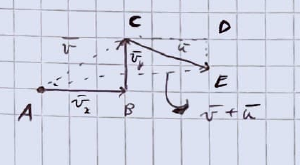
\includegraphics[width=.3\linewidth]{geometria_tex_assets/b41_p45_somma.png}\end{center}
\[\bar v=\|\bar v_x\|(1,0)+\|\bar v_y\|(0,1).\]

% Pagina originale 46
\pagina{46}
\textbf{Vettori liberi nello spazio.} L'insieme di tutti i segmenti orientati nello spazio $\Sigma$ si indica con $S_3$. La relazione di equipollenza rimane invariata a quella presente nel piano.

$V_3$ è uno spazio vettoriale di dimensione 3.
\[\forall\bar x\in V_3:\ \exists(h_1,h_2,h_3)\in\mathbb R^3\text{ tali che }\bar x=h_1\bar v+h_2\bar u+h_3\bar w.\]
Come nelle altre figure geometriche l'importante è che $\bar v,\bar u$ e $\bar w$ siano linearmente indipendenti.

\textbf{Linearità dipendente.} Nella retta l'unico vettore linearmente dipendente è il vettore $\bar0$. Nel piano 2 vettori sono linearmente dipendenti se paralleli. Nello spazio 3 vettori sono linearmente dipendenti se complanari.
\[\mathcal B_1=\{\bar v\}\text{ se }\bar v\ne\bar0,\]
\[\mathcal B_2=\{\bar v,\bar u\}\text{ se }\bar v\not\parallel\bar u,\]
\[\mathcal B_3=\{\bar v,\bar u,\bar w\}\text{ se }\bar v,\bar u,\bar w\text{ non complanari}.\]
Di solito vengono scelti delle basi contenenti vettori ortonormali (ortogonali tra loro e con norma 1).
\[\mathcal B_3=\{\bar i,\bar j,\bar k\},\qquad \bar i=(1,0,0),\quad\bar j=(0,1,0),\quad\bar k=(0,0,1).\]
\begin{center}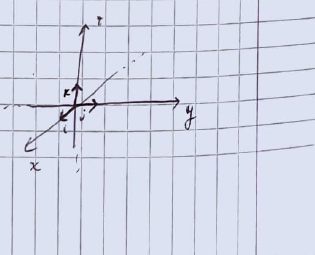
\includegraphics[width=.35\linewidth]{geometria_tex_assets/b41_p46_assi.png}\end{center}
% Pagina originale 47
\pagina{47}
\[\mathcal B_1=\{\bar v\},\qquad\forall\bar x\in V_1:\ \exists h\in\mathbb R\text{ tale che }h\bar v=\bar x.\]
Dimostrazione: $h=\pm\dfrac{\|\bar x\|}{\|\bar v\|}$.
\[\mathcal B_2=\{\bar v,\bar u\},\qquad\forall\bar x\in V_2:\ \exists(h_1,h_2)\in\mathbb R^2\text{ tali che }h_1\bar v+h_2\bar u=\bar x.\]
\[h_1\bar v+h_2\bar u=\bar0\quad\text{con }(h_1,h_2)\ne(0,0),\]
\[\bar v=-\frac{h_2}{h_1}\bar u\Longleftrightarrow\bar v\text{ e }\bar u\text{ paralleli}.\]
\textbf{Prodotti tra vettori.} Si indica con $\widehat{\bar v\bar u}$ l'angolo convesso ($0\le\theta\le\pi$) determinato dai rappresentanti dei 2 vettori applicati nello stesso punto.

\textbf{Prodotto scalare.} Si chiama prodotto scalare il numero reale indicato con $\bar v\cdot\bar u$ (o $\bar v\bar u$), dove
\[\bar v\cdot\bar u=\|\bar v\|\,\|\bar u\|\cos\widehat{\bar v\bar u}.\]
Se $\|\bar v\|=\|\bar u\|=1$, allora $\bar v\cdot\bar u$ indica $\cos\widehat{\bar v\bar u}$.
Se $\|\bar v\|=1$, $\bar v\cdot\bar u$ indica la proiezione di un rappresentante di $\bar u$ sulla retta di $\bar v$.
Se $\bar v=\bar0\lor\bar u=\bar0$, $\bar v\cdot\bar u=0$ per convenzione.
\[\bar v\cdot\bar u=0,\quad\{\bar v,\bar u\}\ne\{\bar0\}\Longrightarrow\bar v\text{ e }\bar u\text{ sono ortogonali (perpendicolari)}.\]

% Pagina originale 48
\pagina{48}
Proprietà:
\begin{enumerate}
\item $\forall\bar v,\bar u\in V_3$: $\bar v\cdot\bar u=\bar u\cdot\bar v$.
\item $\forall\bar v,\bar u,\bar w\in V_3$: $\bar v\cdot(\bar u+\bar w)=\bar v\cdot\bar u+\bar v\cdot\bar w$.
\item $\forall\bar v,\bar u\in V_3$, $\forall h\in\mathbb R$: $h(\bar v\cdot\bar u)=(h\bar v)\cdot\bar u$.
\item $\forall\bar v\in V_3$: $\bar v\cdot\bar v\ge0$.
\item $\forall\bar v\in V_3$: $\bar v\cdot\bar v=0\Longleftrightarrow\bar v=\bar0$.
\end{enumerate}
Siano $\bar i,\bar j,\bar k$ versori ortogonali a 2 a 2:
\[\bar i\cdot\bar i=\bar j\cdot\bar j=\bar k\cdot\bar k=1\cdot1\cos0=1,\]
\[\bar i\cdot\bar j=\bar i\cdot\bar k=\bar j\cdot\bar k=1\cdot1\cos\frac\pi2=0.\]
Siano
\[\bar v=v_1\bar i+v_2\bar j+v_3\bar k,\qquad\bar u=u_1\bar i+u_2\bar j+u_3\bar k.\]
\[\begin{aligned}
\bar v\cdot\bar u={}&v_1u_1\bar i\cdot\bar i+v_1u_2\bar i\cdot\bar j+v_1u_3\bar i\cdot\bar k\\
&+v_2u_1\bar j\cdot\bar i+v_2u_2\bar j\cdot\bar j+v_2u_3\bar j\cdot\bar k\\
&+v_3u_1\bar k\cdot\bar i+v_3u_2\bar k\cdot\bar j+v_3u_3\bar k\cdot\bar k\\
={}&v_1u_1+v_2u_2+v_3u_3,
\end{aligned}\]
quindi $\displaystyle\bar v\cdot\bar u=\sum_{n=1}^3v_nu_n$.
\[\bar v\cdot\bar v=\|\bar v\|\,\|\bar v\|\cos0=\|\bar v\|^2,\qquad \bar v\cdot\bar v=v_1^2+v_2^2+v_3^2,\]
quindi $\|\bar v\|=\sqrt{v_1^2+v_2^2+v_3^2}$.
\[\operatorname{vers}\bar v=\frac1{\|\bar v\|}\bar v\qquad\text{(versore di }\bar v\text{)}.\]
% Pagina originale 49
\pagina{49}
\[\cos\widehat{\bar v\bar u}=\frac{\bar v\cdot\bar u}{\|\bar v\|\,\|\bar u\|}
=\frac{v_1u_1+v_2u_2+v_3u_3}{\sqrt{v_1^2+v_2^2+v_3^2}\sqrt{u_1^2+u_2^2+u_3^2}}.\]
\textbf{Prodotto vettoriale.} Si chiama prodotto vettoriale fra $\bar v$ e $\bar u$, vettori non nulli, e si indica con $\bar v\wedge\bar u$, il vettore che:
\begin{enumerate}\item ha per modulo $\|\bar v\|\,\|\bar u\|\sin\widehat{\bar v\bar u}$;
\item per direzione la direzione ortogonale ai due vettori $\bar v$ e $\bar u$;
\item per verso quello secondo cui il secondo estremo del vettore $\bar v\wedge\bar u$ vede ruotare il vettore $\bar v$ verso il vettore $\bar u$ in senso antiorario con un angolo convesso.\end{enumerate}
\begin{center}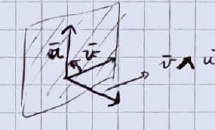
\includegraphics[width=.26\linewidth]{geometria_tex_assets/b41_p49_vettoriale.png}\quad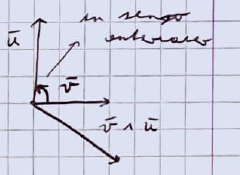
\includegraphics[width=.26\linewidth]{geometria_tex_assets/b41_p49_verso.png}\end{center}
\[\bar v\wedge\bar u=\bar0\Longleftrightarrow\begin{cases}\bar v\text{ è vettore nullo},\\\bar u\text{ è vettore nullo},\\\bar v\parallel\bar u.\end{cases}\]
% La lista originale esprime i tre casi alternativi.
Proprietà:
\begin{enumerate}
\item $\forall\bar v,\bar u\in V_3$: $\bar v\wedge\bar u=-\bar u\wedge\bar v$ (proprietà anticommutativa).
\item $\forall\bar v,\bar u,\bar w\in V_3$: $\bar v\wedge(\bar u+\bar w)=\bar v\wedge\bar u+\bar v\wedge\bar w$ (distributiva).
\item $\forall\bar v,\bar u\in V_3$, $\forall h\in\mathbb R$: $h(\bar v\wedge\bar u)=(h\bar v)\wedge\bar u$.
\end{enumerate}
In generale $(\bar v\wedge\bar u)\wedge\bar w\ne\bar v\wedge(\bar u\wedge\bar w)$: non associatività.

% Pagina originale 50
\pagina{50}
\[\bar i\wedge\bar i=\bar j\wedge\bar j=\bar k\wedge\bar k=0.\]
\[\bar i\wedge\bar j=\bar k,\qquad\bar j\wedge\bar k=\bar i,\qquad\bar k\wedge\bar i=\bar j.\]
\[\bar j\wedge\bar i=+\bar k,\qquad\bar k\wedge\bar j=-\bar i,\qquad\bar i\wedge\bar k=-\bar j.\]
% Refuso originale: j wedge i = +k, invece di -k. Mantenuto.
\[\bar v\wedge\bar u=(u_3v_2-u_2v_3)\bar i-(u_3v_1-u_1v_3)\bar j+(u_2v_1-u_1v_2)\bar k.\]
\[\bar v\wedge\bar u=\begin{vmatrix}\bar i&\bar j&\bar k\\v_1&v_2&v_3\\u_1&u_2&v_3\end{vmatrix}.\]
% Refuso originale: v_3 nell'ultima posizione invece di u_3. Mantenuto.
\textbf{Prodotto misto.} Si definisce prodotto misto tra tre vettori liberi $\bar v,\bar u,\bar w$ dello spazio $V_3$ il numero reale $\bar v\cdot(\bar u\wedge\bar w)$ che corrisponde al determinante della matrice $M$, con
\[M=\begin{pmatrix}v_1&v_2&v_3\\u_1&u_2&u_3\\w_1&w_2&w_3\end{pmatrix},\]
quindi
\[\bar v\cdot(\bar u\wedge\bar w)=\begin{vmatrix}v_1&v_2&v_3\\u_1&u_2&v_3\\w_1&w_2&w_3\end{vmatrix}.\]
% Lo stesso v_3 al posto di u_3 ricompare nel determinante originale.
\textbf{Autovalori.} Si dice che uno scalare $\lambda\in K$ è un autovalore per un endomorfismo $f:V\to V$ se esiste $\bar v\in V^*$ tale che $f(\bar v)=\lambda\bar v$. $\bar v$ è detto autovettore.
L'autospazio è l'insieme di tutti i vettori per cui $f(\bar v)=\lambda\bar v$ ($\bar0\in V_\lambda$, ma $\bar0$ non è autovettore).
\[V_\lambda=\{\bar v\in V\mid f(\bar v)=\lambda\bar v\}.\]
% Pagina originale 51
\pagina{51}
$V_\lambda$ è un sottospazio di $V$. Contiene sempre $\bar0$ e verifica le proprietà di chiusura:
\[f(\bar v_1)+f(\bar v_2)=\lambda\bar v_1+\lambda\bar v_2=\lambda(\bar v_1+\bar v_2)=f(\bar v_1+\bar v_2),\]
\[kf(\bar v)=k\lambda\bar v=\lambda k\bar v=f(k\bar v).\]
\[L(\bar v_1,\bar v_2,\ldots,\bar v_m)\subseteq V_\lambda,\qquad\bar v_1,\bar v_2,\ldots,\bar v_m\in V_\lambda.\]
0 può essere autovalore se in questo caso $\ker f\ne\{\bar0\}$, quindi $f$ non è iniettiva.
Se $\bar v$ è un autovettore per un certo scalare, $\bar v$ ed $f(\bar v)$ sono paralleli.

\textbf{$V_\lambda\cap V_\mu=\{\bar0_V\}$.}
Dimostrazione:
\[\begin{cases}\bar v\in V_\lambda\Longrightarrow f(\bar v)=\lambda\bar v,\\\bar v\in V_\mu\Longrightarrow f(\bar v)=\mu\bar v,\end{cases}\Longrightarrow\lambda\bar v=\mu\bar v\Longrightarrow(\lambda-\mu)\bar v=\bar0.\]
Quindi $\lambda=\mu\lor\bar v=\bar0$; la prima contraddice le ipotesi.

$\bar u\in V_\lambda$, $\bar w\in V_\mu$ sono linearmente indipendenti.
Se $a\bar u+b\bar w=\bar0\Longrightarrow\bar u=-\dfrac ba\bar w\Longrightarrow\bar u\in V_\mu$.
\[f\left(-\frac ba\bar w\right)=\lambda\left(-\frac ba\right)\bar w=\left(-\frac ba\right)(\lambda\bar w)=-\frac ba f(\bar w).\]
% Originale: lambda scritto anche nel termine che coinvolge w in V_mu; mantenuto.
$\mathcal B_{V_\lambda}\cup\mathcal B_{V_\mu}\cup\cdots\cup\mathcal B_{V_\sigma}$ forma un sottoinsieme di vettori linearmente indipendenti.

% Pagina originale 52
\pagina{52}
\textbf{Matrici simili.} Siano $A$ e $B$ matrici di $K^{n,n}$. $A$ e $B$ sono matrici simili se
\[\exists P\in K^{n,n},\quad |P|\ne0,\quad\text{tale che }B=P^{-1}AP.\]
Conviene osservare che $P$ non è unica.
La relazione di similitudine è una relazione di equivalenza.
La proprietà riflessiva si verifica usando $P$ (matrice di passaggio) $=I_n$:
\[A=I_n^{-1}AI_n=I_nAI_n=AI_n=A.\]
La proprietà simmetrica invece si verifica così:
\[B=P^{-1}AP\Longrightarrow PB=PP^{-1}AP\Longrightarrow PB=AP\]
\[\Longrightarrow PBP^{-1}=APP^{-1}\Longrightarrow PBP^{-1}=A.\]
E $P'=P^{-1}\Longrightarrow A=(P')^{-1}BP'$.
Infine c'è la proprietà transitiva:
\[B=P^{-1}AP\land C=Q^{-1}BQ,\]
\[C=Q^{-1}BQ=Q^{-1}(P^{-1}AP)Q=(Q^{-1}P^{-1})A(PQ).\]
$S=PQ\Longrightarrow C=S^{-1}AS$.
\[A\text{ simile a }B\Longrightarrow r(A)=r(B).\]
\textbf{Matrice diagonalizzabile.} Una matrice $A$ è diagonalizzabile se simile ad una matrice diagonale.
% Pagina originale 53
\pagina{53}
\textbf{Autovalori per una matrice.} Si dice che uno scalare $\lambda$ è autovalore per una matrice di $K^{n,n}$ se
\[\exists X\in K^{n,1}\text{ non nullo tale che }AX=\lambda X.\]
$X$ è detto autovettore. $V_\lambda$ è l'autospazio che contiene il vettore colonna nullo. $V_\lambda\subseteq K^{n,1}$ perché rispetta le 2 proprietà di chiusura:
\begin{enumerate}\item $A(X+Y)=AX+AY=\lambda X+\lambda Y=\lambda(X+Y)$;
\item $A(hX)=h(AX)=h(\lambda X)=\lambda(hX)$.\end{enumerate}
\[AX=\lambda X\Longrightarrow(A-\lambda I_n)X=O_{n,1}.\]
\textbf{Polinomio caratteristico.} Si chiama polinomio caratteristico di una matrice $A$ $|A-\lambda I_n|$. Si chiama \textbf{equazione caratteristica} l'equazione
\[|A-\lambda I_n|=0.\]
Il polinomio sarà di grado $n$ ed avrà $(-1)^n\lambda^n$, quindi avrà al massimo $n$ soluzioni. Il polinomio sarà di tipo
\[(-1)^n\lambda^n+(-1)^{n-1}\operatorname{tr}(A)\lambda^{n-1}+\cdots+|A|.\]
\textbf{$A$ e $B$ simili $\Longrightarrow$ stesso polinomio caratteristico.}
\[\begin{aligned}
|B-\lambda I_n|&=|P^{-1}AP-\lambda I_n|=|P^{-1}AP-\lambda P^{-1}I_nP|\\
&=|P^{-1}AP-P^{-1}\lambda I_nP|=|P^{-1}(A-\lambda I_n)P|\\
&=|P^{-1}|\,|A-\lambda I_n|\,|P|=|A-\lambda I_n|.
\end{aligned}\]

% Pagina originale 54
\pagina{54}
L'equazione caratteristica di $A$ è anche:
\[(-1)^nA^n+a_{n-1}A^{n-1}+\cdots+a_2A^2+a_1A+a_0I_n=O_{n,n},\]
che può essere usata per trovare la matrice inversa:
\[A^{-1}\bigl((-1)^nA^n+a_{n-1}A^{n-1}+\cdots+a_2A^2+a_1A+a_0I_n\bigr)=A^{-1}O_{n,n},\]
quindi
\[(-1)^nA^{n-1}+a_{n-1}A^{n-2}+\cdots+a_2A+a_1I_n+a_0A^{-1}=O_{n,n},\]
\[(-1)^nA^{n-1}+a_{n-1}A^{n-2}+\cdots+a_2A+a_1I_n=-a_0A^{-1},\]
\[A^{-1}=-\frac1{a_0}\bigl[(-1)^nA^{n-1}+a_{n-1}A^{n-2}+\cdots+a_2A+a_1I_n\bigr].\]
Sussistono le proprietà degli autovalori / autospazi / autovettori:
\begin{enumerate}\item $V_\mu\cap V_\lambda=\{\bar0_V\}$;
\item $X\in V_\mu$, $Y\in V_\lambda\Longrightarrow X$ e $Y$ linearmente indipendenti;
\item $\displaystyle\bigcup_{i\text{-esimo autovalore}}\mathcal B_{V_i}$ è un sottoinsieme di vettori linearmente indipendenti.
\end{enumerate}
\textbf{Molteplicità algebrica.} Sia $A$ una matrice e $\lambda$ suo autovalore; si chiama molteplicità algebrica di $\lambda$ la sua molteplicità nelle soluzioni dell'equazione caratteristica.

\textbf{Molteplicità geometrica.} Sia $A$ matrice e $\lambda$ suo autovalore; si chiama molteplicità geometrica di $\lambda$ la dimensione del sottospazio $V_\lambda$.
\[1\le\dim V_\lambda\le m_a(\lambda),\]
cioè la molteplicità algebrica è sempre maggiore di quella geometrica.
% Pagina originale 55
\pagina{55}
\[\dim V_\lambda=n-r(A-\lambda I_n),\qquad n=\text{ordine di }A.\]
$A$ è diagonalizzabile se e solo se:
\begin{enumerate}\item tutte le soluzioni sono autovalori ($\in K$);
\item $\dim V_\lambda=m_a(\lambda)$ (molteplicità algebrica corrisponde a quella geometrica).\end{enumerate}
Le matrici reali simmetriche sono sempre diagonalizzabili.

Due matrici sono simili se e solo se:
\begin{enumerate}\item hanno gli stessi autovalori;
\item stessa molteplicità algebrica;
\item stessa molteplicità geometrica.\end{enumerate}
% La condizione di similitudine è riportata come nell'originale (non è sufficiente in generale).
$A$ è diagonalizzabile se esiste una base formata solo da autovettori di $K^{n,1}$.

Se $A$ diagonalizzabile, la matrice di passaggio è formata dalle basi di $K^{n,1}$ formate dagli autovettori.

% Pagina originale 56
\pagina{56}
\textbf{Geometria nel piano.}

\textbf{Riferimento cartesiano.} Si chiama riferimento cartesiano e si indica $\mathcal R=(O,\mathcal B)$ una coppia ordinata costituita da un punto $O$ detto origine e una base $\mathcal B$ dello spazio vettoriale $V_n$.

\textbf{Nella retta.} Si chiama riferimento cartesiano e si indica $\mathcal R=(O,\mathcal B)$ una coppia ordinata costituita da un punto $O$ detto origine e una base $\mathcal B$ dello spazio vettoriale $V_1$.
A ciascun punto viene associato un numero reale che è la componente del vettore $\overrightarrow{OP}$ rispetto alla base $\mathcal B$ di $\mathcal R$ ed è chiamata ascissa del punto (coordinata).
Sia $\bar u_1$ il vettore che forma la base $\mathcal B$:
\[\overrightarrow{OA}=x_1\bar u_1,\qquad\overrightarrow{OB}=x_2\bar u_1,\]
dove $x_1,x_2$ sono le ascisse di $\overrightarrow{OA}$ e $\overrightarrow{OB}$.
\[\overrightarrow{AB}=\overrightarrow{OB}-\overrightarrow{OA}=x_2\bar u_1-x_1\bar u_1=\bar u_1(x_2-x_1).\]
\textbf{Punto medio.} Nella retta il punto medio $M$ tra 2 punti distinti $A$ e $B$ ha come ascissa $\dfrac{x_1+x_2}{2}$.
Dimostrazione:
\[x-x_1=x_2-x_2\Longrightarrow x=\frac{x_1+x_2}{2}.\]
% Refuso nella dimostrazione originale: x_2-x_2 al posto di x_2-x.
% Pagina originale 57
\pagina{57}
\textbf{Punto simmetrico.} Siano $A$ ed $M$ due punti della retta; il simmetrico $B$ di $A$ rispetto ad $M$ ha ascissa
\[x_2=2x-x_1,\qquad A\leftrightarrow x_1,\ M\leftrightarrow x,\ B\leftrightarrow x_2.\]
\textbf{Nel piano.} Si chiama riferimento cartesiano la coppia ordinata $\mathcal R=(O,\mathcal B)$ che ha come prima componente un punto $O$ detto origine e $\mathcal B$ base dello spazio vettoriale $V_2$.
Ogni punto ha una coppia di numeri reali associati ad esso chiamati rispettivamente ascissa e ordinata.
Solitamente viene scelta la base canonica $\mathcal B=\{\bar i,\bar j\}$ ed in tal caso $\mathcal R$ è un riferimento metrico (o monometrico ortogonale).
\[\overrightarrow{OA}=x_1\bar i+y_1\bar j,\qquad\overrightarrow{OB}=x_2\bar i+y_2\bar j,\]
\[\overrightarrow{AB}=\overrightarrow{OB}-\overrightarrow{OA}=(x_2-x_1)\bar i+(y_2-y_1)\bar j.\]
Il punto medio $M$ tra 2 punti $A$ e $B$ ha come coordinate
\[\left(\frac{x_1+x_2}{2},\frac{y_1+y_2}{2}\right).\]
Si dimostra con $x-x_1=x_2-x$, $y-y_1=y_2-y$.

\textbf{Nello spazio.} Si chiama riferimento cartesiano nello spazio la coppia ordinata $\mathcal R=(O,\mathcal B)$ costituita da un punto $O$ detto origine e una base $\mathcal B$ dello spazio vettoriale $V_3$.

% Pagina originale 58
\pagina{58}
Ad ogni punto viene associata una terna ordinata di numeri reali $(x,y,z)$ dove $x$ è l'ascissa, $y$ è l'ordinata e $z$ è la quota.
Solitamente viene scelta come base di riferimento $\{\bar i,\bar j,\bar k\}$. In questo caso il riferimento è metrico (o monometrico ortogonale).
\[\overrightarrow{OA}=x_1\bar i+y_1\bar j+z_1\bar k,\qquad\overrightarrow{OB}=x_2\bar i+y_2\bar j+z_2\bar k,\]
\[\overrightarrow{AB}=\overrightarrow{OB}+\overrightarrow{OA}=(x_2-x_1)\bar i+(y_2-y_1)\bar j+(z_2-z_1)\bar k.\]
% Originale: OB+OA, mentre le coordinate riportate corrispondono a OB-OA.
Il punto medio $M$ ha come coordinate la terna
\[\left(\frac{x_1+x_2}{2},\frac{y_1+y_2}{2},\frac{z_1+z_2}{2}\right),\]
che si possono dedurre da
\[x-x_1=x_2-x,\qquad y-y_1=y_2-y,\qquad z-z_1=z_2-z.\]
\textbf{Equazione parametrica della retta nello spazio.} Si prende un punto $P_0(x_0,y_0,z_0)\in r$ con direzione nota indicata da $\bar v=(l,m,n)$ che è parallelo alla retta $r$.
Le coordinate di $P\in r$ devono far sì che il vettore $\overrightarrow{PP_0}$ sia parallelo alla retta $r$, cioè
\[\exists t\in\mathbb R\text{ tale che }\overrightarrow{PP_0}=t\bar v,\quad\text{cioè}\quad\begin{cases}x-x_0=tl,\\y-y_0=tm,\\z-z_0=tn.\end{cases}\]
% Nell'originale il vettore è PP_0, ma le componenti sono P-P_0: mantenuto.
Questa equazione vale anche per spazi vettoriali $V_n$ con $\dim V_n=n\ge3$.
% Pagina originale 59
\pagina{59}
\textbf{Allineamento di 3 punti.} Siano $A(x_1,y_1,z_1)$, $B(x_2,y_2,z_2)$ e $C(x_3,y_3,z_3)$ 3 punti distinti nello spazio; $A,B,C$ sono allineati se i vettori rappresentanti sono paralleli, cioè la matrice $A$ ha rango 1.
\[r\begin{pmatrix}x_3-x_1&y_3-y_1&z_3-z_1\\x_2-x_1&y_2-y_1&z_2-z_1\end{pmatrix}=1.\]
\textbf{Equazione della retta sotto forma di rapporti uguali.}
\[\frac{x-x_1}{x_2-x_1}=\frac{y-y_1}{y_2-y_1}=\frac{z-z_1}{z_2+z_1}.\]
% L'ultimo denominatore sembra z_2+z_1 nell'originale; mantenuto.
Se uno dei denominatori è nullo, per convenzione $\dfrac{a-a_1}{a_2-a_1}$ con $a_1=a_2$ diventa $a_1=a_2$ nella tripla equazione, cioè
\[\begin{cases}x_1=x_2,\\\dfrac{y-y_1}{y_2-y_1}=\dfrac{z-z_1}{z_2-z_1},\end{cases}\qquad y_2-y_1=m,\quad z_2-z_1=n,\quad x_2-x_1=l.\]
% Anche x_1=x_2 è scritto così nel caso degenere originale.
\textbf{Parametri direttori.} Si chiamano parametri direttori (o numeri direttori) le componenti di un vettore non nullo parallelo alla retta stessa. Nel caso il vettore $\bar v$ sia un versore ($\|\bar v\|=1$), i parametri direttori prendono il nome di \textbf{coseni direttori}. Questo perché
\[\bar v\cdot\bar i=\|\bar v\|\,\|\bar i\|\cos\widehat{\bar v\bar i}=\cos\widehat{\bar v\bar i},\]
\[\bar v\cdot\bar i=l,\quad\text{da cui segue che }l=\cos\widehat{\bar v\bar i}.\]

% Pagina originale 60
\pagina{60}
\textbf{Rappresentazione della retta nel piano.}
\[\begin{cases}x-x_0=tl,\\y-y_0=tm,\end{cases}\qquad\text{rappresentazione parametrica}.\]
\[t=\frac{x-x_0}{l}=\frac{y-y_0}{m}\qquad\text{rappresentazione mediante rapporti uguali}.\]
Se $m=0\Longrightarrow y=y_0$. Se $l=0\Longrightarrow x=x_0$.
\[\frac{x-x_0}{l}=\frac{y-y_0}{m}\Longrightarrow m(x-x_0)-l(y-y_0)=0,\]
che si riconduce alla forma $ax+by+c=0$: equazione implicita.
\[a=m,\qquad b=-l,\qquad c=ly_0-mx_0.\]
Con $a=1$, $b=0$, $c=-x_0$ si ha $x-x_0=0$.
Con $a=0$, $b=1$, $c=-y_0$ si ha $y-y_0=0$.
\[ax+by+c=0\Longrightarrow y=-\frac abx-\frac cb\qquad\text{equazione esplicita}.\]
$-\dfrac ab$ è il coefficiente angolare, $-\dfrac cb$ l'ascissa sull'asse $x$.
% L'originale descrive -c/b come ascissa sull'asse x; mantenuto.
Punto generico nella retta: $P(x_0+lt,y_0+mt)$.
Sia $\bar n=(a,b)\perp r$, $P_0\in r$:
\[a(x-x_0)+b(y-y_0)=0\qquad\bigl(\text{cioè }\langle\bar n,\overrightarrow{PP_0}\rangle=0\bigr).\]
\textbf{Intersezioni e parallelismo tra 2 rette di un piano.}
Siano $r$ ed $s$ 2 rette giacenti nel piano $\pi$, con
\[r:ax+by+c=0,\qquad s:a'x+b'y+c'=0.\]

% Pagina originale 61
\pagina{61}
Il sistema $\begin{cases}ax+by+c=0,\\a'x+b'y+c'=0\end{cases}$ è un sistema di Cramer se e solo se
\[\begin{vmatrix}a&b\\a'&b'\end{vmatrix}\ne0.\]
In questo caso il sistema ammette un'unica soluzione e quindi le rette risultano incidenti.
Se $\begin{vmatrix}a&b\\a'&b'\end{vmatrix}=0$, allora:
\begin{itemize}
\item $r\begin{pmatrix}a&b&-c\\a'&b'&-c'\end{pmatrix}=1\Longrightarrow r\parallel s$ e coincidenti ($r=s$);
\item $r\begin{pmatrix}a&b&-c\\a'&b'&-c'\end{pmatrix}=2\Longrightarrow r\parallel s$ e distinte.
\end{itemize}
In entrambi i casi $\begin{vmatrix}a&b\\a'&b'\end{vmatrix}=0\Longleftrightarrow r\parallel s$, cioè $ax+by+c=0\parallel ax+by+k=0$, con la stessa coppia di direttori $(-b,a)$, $\forall k\in\mathbb R$.
\textbf{Fascio proprio di rette.} È la rappresentazione simultanea di tutte le rette del piano passanti per il punto $P(x_0,y_0)$, del tipo
\[a(x-x_0)+b(y-y_0)=0,\]
dove le scelte dei parametri direttori $(-b,a)$ [o $(b,-a)$] hanno unica condizione $(a,b)\ne(0,0)$.
Ciò è equivalente a $\dfrac{x-x_0}{l}=\dfrac{y-y_0}{m}$ con $(l,m)=(-b,a)$ o $(b,-a)$.
\begin{center}
\setlength{\unitlength}{1mm}
\begin{picture}(36,25)
\put(4,3){\line(1,1){22}}\put(4,25){\line(1,-1){22}}
\put(15,14){\circle*{1}}\put(17,14){$P$}
\end{picture}
\end{center}
Si può usare anche la forma esplicita $y-y_0=m(x-x_0)$, che esclude le rette parallele all'asse delle ordinate.
% Pagina originale 62
\pagina{62}
\textbf{Rette perpendicolari.} Siano $r$ ed $s$ due rette ed $\bar r$ ed $\bar s$ i parametri direttori:
\[r\perp s\Longleftrightarrow\langle\bar r,\bar s\rangle=0,\]
cioè $\bar r\cdot\bar s=\|\bar r\|\|\bar s\|\cos\widehat{\bar r\bar s}=0$, o anche $l_1l_2+m_1m_2=0$.
\textbf{Distanze nel piano.}
\[d(A,B)=\|\overrightarrow{AB}\|=\sqrt{(x_2-x_1)^2+(y_2-y_1)^2}.\]
Questa formula può essere usata per calcolare la distanza tra due rette parallele, ad esempio.
\begin{center}
\setlength{\unitlength}{1mm}
\begin{picture}(55,34)
\put(4,10){\line(2,1){38}}\put(4,0){\line(2,1){38}}
\put(13,32){\line(1,-2){14}}
\put(19,17.5){\circle*{1}}\put(23,9.5){\circle*{1}}
\put(15,19){$P$}\put(24,7){$H$}\put(43,28){$r$}\put(43,18){$s$}\put(28,2){$n\perp r$}
\end{picture}
\end{center}
Siano $P$ un punto $\in r$ ed $(a,b)$ direttori di $n$, allora
\[n:\begin{cases}x-x_0=at,\\y-y_0=bt.\end{cases}\]
Si sostituisce ad $s$ l'equazione generica di $H\in n\cap s$, $(x_0+at,y_0+bt)$, quindi
\[a(x_0+at)+b(y_0+bt)+c=0,\]
e risolvo per trovare il valore di $t$: $t_H=-\dfrac{ax_0+by_0+c}{a^2+b^2}$.
Si ottengono così le coordinate di $H(x_0+at_H,y_0+bt_H)$.
\begin{align*}
d(P,H)&=\sqrt{(x_0+at_H-x_0)^2+(y_0+bt_H-y_0)^2}\\
&=\sqrt{a^2t_H^2+b^2t_H^2}=|t_H|\sqrt{a^2+b^2},
\end{align*}
cioè $\left|-\dfrac{ax_0+by_0+c}{a^2+b^2}\right|\sqrt{a^2+b^2}=\dfrac{|ax_0+by_0+c|}{\sqrt{a^2+b^2}}$.
% Pagina originale 63
\pagina{63}
\textbf{Coniche.}
\[ax^2+byx+cy^2+dx+ey+f=0,\]
cioè $a_{11}x^2+2a_{12}xy+a_{22}y^2+2a_{13}x+2a_{23}y+a_{33}=0$.
\[A=\begin{pmatrix}a_{11}&a_{12}&a_{13}\\a_{21}&a_{22}&a_{23}\\a_{31}&a_{32}&a_{33}\end{pmatrix}
=\begin{pmatrix}a&b/2&d/2\\b/2&c&e/2\\d/2&e/2&f\end{pmatrix}.\]
% Originale: matrice intermedia riscritta e corretta a fianco; riportata la versione finale.
Esempio: $y=ax^2\Longrightarrow ax^2-y=0$ corrisponde ad
\[A=\begin{pmatrix}a&0&0\\0&0&-1/2\\0&-1/2&0\end{pmatrix}.\]
\textbf{Equazioni di un piano.} Per ricavare l'equazione di un piano possiamo immaginare di avere $P_0\in\pi$ ed $\bar n$ tale che $\bar n\perp\pi$ (la retta a cui appartiene tale vettore $\bar n$), con $P\in\pi$ punto generico.
\[\bar n\perp\pi\Longleftrightarrow\bar n\perp\overrightarrow{PP_0},\]
cioè $\langle\bar n,\overrightarrow{PP_0}\rangle=0\Longleftrightarrow a(x-x_0)+b(y-y_0)+c(z-z_0)=0$,
\[\Longrightarrow ax+by+cz+d=0,\qquad d=-ax_0-by_0-cz_0.\]
Avendo tre punti $A,B,C$, $\overrightarrow{AB}\wedge\overrightarrow{BC}$ dà come risultato un vettore ortogonale al piano.
\textbf{Intersezioni e parallelismo tra piani.} Siano $\pi:ax+by+cz+d=0$, $\pi':a'x+b'y+c'z+d'=0$ due piani nello spazio, allora
\[r\begin{pmatrix}a&b&c&d\\a'&b'&c'&d'\end{pmatrix}=2\Longleftrightarrow\pi\text{ e }\pi'\text{ incidenti}\]
(l'intersezione è una retta, $\infty^1$).
% Refuso originale p63: è usata la matrice completa nel criterio, che include anche piani paralleli distinti.
% Pagina originale 64
\pagina{64}
\[r\begin{pmatrix}a&b&c&d\\a'&b'&c'&d'\end{pmatrix}=1\Longleftrightarrow\pi\parallel\pi'.\]
% Originale: riporta d,d' nella matrice del criterio di parallelismo; mantenuto.
Se $r\begin{pmatrix}a&b&c\\a'&b'&c'\end{pmatrix}=1$, i piani sono paralleli e distinti oppure paralleli e coincidenti.
Una retta nello spazio può essere sempre rappresentata come l'intersezione tra due piani.
L'insieme di tutti i piani distinti contenenti una retta $r$ si chiama \textbf{fascio proprio di piani di asse $r$}.
Una terna di direttori della retta è $(bc'-b'c,\ a'd-ac',\ ab'-a'b)$.
% Pagina 64: secondo termine a'd-ac' (invece del consueto ca'-ac'); mantenuto.
Il vettore $\bar n(a,b,c)\perp\pi$ e $\bar n'(a',b',c')\perp\pi'$: $\bar n\wedge\bar n'\parallel r$.
\textbf{Fasci propri e impropri di piani.}
\[r:\begin{cases}\pi,\\\pi',\end{cases}\qquad A_r=\begin{pmatrix}a&b&c&d\\a'&b'&c'&d'\end{pmatrix},\qquad r(A_r)=2.\]
Con $(\lambda,\mu)\ne(0,0)$,
\[\lambda(ax+by+cz+d)+\mu(a'x+b'y+c'z+d')=0\]
è l'equazione del fascio proprio di piani che contiene $r$.
Sia $P_1(x_1,y_1,z_1)\in r$, allora
\[\lambda(ax_1+by_1+cz_1+d)+\mu(a'x_1+b'y_1+c'z_1+d')=0,\]
cioè $\lambda\cdot0+\mu\cdot0=0$.
% Pagina originale 65
\pagina{65}
L'equazione può essere riscritta come
\[(\lambda a+\mu a')x+(\lambda b+\mu b')y+(\lambda c+\mu c')z+(\lambda d+\mu d')=0,\]
\[\begin{cases}\lambda a+\mu a'=0,\\\lambda b+\mu b'=0,\\\lambda c+\mu c'=0.\end{cases}\]
$\pi_{\parallel}:ax+by+cz+k=0$ è l'equazione del piano parallelo a $\pi$ generico, con $k\in\mathbb R$.
\textbf{Intersezione tra piano e retta.} Siano $\pi:ax+by+cz+d=0$ piano e
\[r:\begin{cases}x=x_0+lt,\\y=y_0+mt,\\z=z_0+nt.\end{cases}\]
$P\in r\cap\pi$ è un punto che soddisfa
\[a(x_0+lt)+b(y_0+mt)+c(z_0+nt)+d=0\]
\[\Longrightarrow(al+bm+cn)t+(ax_0+by_0+cz_0+d)=0\]
\[\Longrightarrow t=-\frac{ax_0+by_0+cz_0+d}{al+bm+cn}\qquad\text{se }al+bm+cn\ne0.\]
Se $al+bm+cn=0$:
\begin{enumerate}
\item se $ax_0+by_0+cz_0+d=0$, allora $r\subset\pi$;
\item se $ax_0+by_0+cz_0+d\ne0$, allora $r$ e $\pi$ sono distinti, non s'incontrano.
\end{enumerate}
$al+bm+cn=0\Longleftrightarrow r\parallel\pi$.
% Pagina originale 66
\pagina{66}
\textbf{Rette complanari e sghembe.} Due rette sono complanari se esiste un piano che le contenga. Se non esiste allora sono sghembe. Se due rette sono complanari possono essere incidenti o parallele.
Rette sghembe non hanno parametri direttori proporzionali.
\[\text{Due rette sono complanari se }\bar v\cdot(\bar u\wedge\bar w)=0,\]
\[\text{Due rette sono sghembe se }\bar v\cdot(\bar u\wedge\bar w)\ne0,\]
dove $\bar v$ è un rappresentante del segmento $AB$ ($A\in r$, $B\in s$), $\bar u$ è un vettore parallelo alla retta $r$, $\bar w$ vettore parallelo alla retta $s$.
\textbf{Angoli tra rette nello spazio e tra piani.}
$\bar n$: parametri direttori di $r$; $\bar n'$: parametri direttori di $s$.
\[\cos\widehat{rs}=\frac{\langle\bar n,\bar n'\rangle}{\|\bar n\|\|\bar n'\|}.\]
Se $r\perp s\Longleftrightarrow\bar n\perp\bar n'\Longrightarrow\langle\bar n,\bar n'\rangle=0$.
$\pi:ax+by+cz+d=0$ ha $\bar n(a,b,c)$ come parametro direttore del piano $\pi$ (un vettore non nullo perpendicolare al piano $\pi$).
% Pagina originale 67
\pagina{67}
\[\cos\widehat{\pi\pi'}=\frac{\langle\bar n,\bar n'\rangle}{\|\bar n\|\|\bar n'\|}=0\Longleftrightarrow\langle\bar n,\bar n'\rangle=0,\]
cioè $aa'+bb'+cc'=0$.
Una retta è parallela ad un piano se $\langle\bar n_r,\bar n_\pi\rangle=0$:
\[r\parallel\pi\Longleftrightarrow\langle\bar n_r,\bar n_\pi\rangle=0,\qquad\text{cioè }al+bm+cn=0.\]
\[r\begin{pmatrix}a&b&c\\l&m&n\end{pmatrix}=1\Longleftrightarrow r\perp\pi.\]
\textbf{Distanza nello spazio.}
\[d(A,B)=\sqrt{(x_B-x_A)^2+(y_B-y_A)^2+(z_B-z_A)^2}.\]
In maniera analoga alla distanza tra punto e retta nel piano possiamo trovare le formule per la distanza tra $P$ e $\pi$:
$P\in n$, con $n\perp r$, cioè $P(x_0+at,y_0+bt,z_0+ct)$ deve soddisfare
\[a(x_0+at)+b(y_0+bt)+c(z_0+ct)+d=0,\]
cioè $(a^2+b^2+c^2)t+(ax_0+by_0+cz_0+d)=0$, quindi
\[t_H=-\frac{ax_0+by_0+cz_0+d}{a^2+b^2+c^2}.\]
% Originale p67: n perpendicolare a r, anche se la distanza è da un piano.
\begin{align*}
d(P,H)&=\sqrt{(x_0+at_H-x_0)^2+(y_0+bt_H-y_0)^2+(z_0+ct_H-z_0)^2}\\
&=|t_H|\sqrt{a^2+b^2+c^2}\\
&=\frac{|ax_0+by_0+cz_0+d|}{\sqrt{a^2+b^2+c^2}}=d(P,\pi).
\end{align*}
% P67: componente z nella penultima radice poco nitida; resa coerente con i passaggi precedenti.
% Pagina originale 68
\pagina{68}
\textbf{Minima distanza e retta di minima distanza tra due rette sghembe.}
L'insieme $D(r,s)=\{d(P,Q)\mid P\in r\land Q\in s\}$ nel caso di $r\parallel s$ ha solo un elemento.
% Affermazione originale p68 mantenuta; le distanze di punti arbitrari su rette parallele non formano un singleton.
Nel caso di $r$ ed $s$ sghembe ha infiniti elementi ed ha un minimo.
Si chiama minima distanza tra due rette $r,s$ il minimo tra le distanze tra due punti $P\in r$ ed $Q\in s$, cioè $\min D(r,s)$.
La retta passante per questi due punti si chiama retta di minima distanza tra le due rette sghembe.
La retta di minima distanza è l'unica retta che interseca entrambe le rette $r,s$ ed è ortogonale ad entrambe.
\end{document}
